\documentclass[3p,times,twocolumn]{elsarticle}

\usepackage{amsmath,amssymb}
\usepackage{graphicx}
\usepackage{booktabs}
\usepackage{array}
\usepackage{multirow}
\usepackage{caption}
\usepackage[T1]{fontenc}
\usepackage[utf8]{inputenc}
\usepackage{textcomp}
\usepackage{xcolor}
\usepackage{hyperref}
\hypersetup{colorlinks=true,linkcolor=blue,citecolor=blue,urlcolor=blue}

\journal{Informatics in Medicine Unlocked / Artificial Intelligence in Medicine}

\newcommand{\ie}{i.e.,}
\newcommand{\eg}{e.g.,}

\begin{document}

\begin{frontmatter}

\title{A Community-Aware Explainable Machine Learning Framework for Childhood Pneumonia Prediction: Feature Ablation, Community Exposure Risk Score Optimization, Calibration, Decision Curve Analysis, and Fairness Evaluation for Low-Resource Community Screening}

\author[a]{Md Artad Chowdhury}
\author[a]{Bishal Paul}

\address[a]{Department of Computer Science and Engineering, [University Name], [City], Bangladesh}

\begin{abstract}
Childhood pneumonia is the leading infectious cause of mortality in children under five years of age, responsible for approximately 700{,}000 deaths annually, with over 95\% of cases occurring in low- and middle-income countries (LMICs). This paper presents the Community-Aware Explainable Pneumonia Prediction Framework (CAEPPF), a comprehensive, clinically grounded machine learning (ML) framework developed and validated on 799 pediatric patients admitted to a tertiary hospital in Rabat, Morocco. CAEPPF integrates nine methodological components that, to our knowledge, have not previously been reported together in the pediatric pneumonia ML literature: (1) a feature ablation study quantifying the incremental discriminative contribution of socio-environmental variables (+1.8 AUC points, 0.861~$\rightarrow$~0.879); (2) data-driven optimization of a novel Community Exposure Risk Score (CERS) using logistic regression coefficients; (3) benchmarking of eleven supervised ML algorithms under a leakage-free Synthetic Minority Oversampling Technique (SMOTE) pipeline with hyperparameter tuning, achieving a Random Forest cross-validated AUC of 0.887 (95\% CI: 0.825--0.949); (4) DeLong and McNemar statistical comparison tests across all top-model pairs; (5) full probability calibration analysis (Brier Score, Expected Calibration Error) identifying Random Forest as the best-calibrated model (Brier~=~0.109, ECE~=~0.052); (6) Decision Curve Analysis demonstrating positive net clinical benefit across relevant decision thresholds; (7) fairness analysis across six demographic subgroups (AUC range 0.846--0.962, no catastrophic performance collapse); (8) expanded SHAP (SHapley Additive exPlanations) interpretability, including dependence and individual waterfall plots; and (9) a sensitivity analysis confirming result stability across ten random seeds. These contributions are integrated into a five-step Clinical Decision Framework featuring a deployable Community Pneumonia Screening Score (CPSS), translating model outputs into actionable triage guidance for community health workers (CHWs) operating without laboratory infrastructure.
\end{abstract}

\begin{keyword}
Childhood pneumonia \sep Machine learning \sep Feature ablation \sep Community Exposure Risk Score \sep SMOTE \sep SHAP \sep Probability calibration \sep Decision curve analysis \sep DeLong test \sep Fairness analysis \sep Household crowding \sep Vaccination \sep Low- and middle-income countries \sep Community health worker
\end{keyword}

\end{frontmatter}

%======================================================================
\section{Introduction}
%======================================================================
Pneumonia is the leading infectious cause of death in children under five years of age worldwide, claiming approximately 700{,}000 lives annually, with over 95\% of cases concentrated in low- and middle-income countries (LMICs) \cite{ref1,ref2,ref3,ref4}. The diagnostic and management gap between high-resource and resource-constrained settings is particularly acute: laboratory biomarkers, chest radiography, and specialist clinical assessment that anchor diagnosis in high-income settings are frequently unavailable to the community health workers (CHWs) and primary care clinicians who serve as the first point of contact for febrile children in LMIC settings \cite{ref10,ref12}.

Machine learning (ML) has emerged as a powerful approach for structured-data risk prediction, offering the capacity to integrate heterogeneous predictors -- clinical biomarkers, demographic variables, and socio-environmental determinants -- into probabilistic risk estimates that could inform triage decisions in resource-limited settings. However, the ML literature on pediatric pneumonia suffers from four persistent methodological gaps: (1) absence of feature ablation studies quantifying the independent contribution of socio-environmental determinants over clinical baselines; (2) reliance on expert-defined rather than data-optimized composite risk indices; (3) omission of clinical validity assessments including probability calibration and decision curve analysis, increasingly required by medical AI reviewers; and (4) lack of fairness evaluation across demographic subgroups, despite growing recognition of algorithmic bias in clinical prediction models.

This paper addresses all four gaps simultaneously through the Community-Aware Explainable Pneumonia Prediction Framework (CAEPPF) -- an integrated research and deployment framework built on a clinical pediatric dataset of 799 children. The framework is named to reflect its three distinguishing properties: \textit{community-awareness} (explicit encoding and quantification of household crowding, vaccination, and passive smoking as structured ML features), \textit{explainability} (grouped SHAP importance, dependence plots, and individual waterfall explanations), and \textit{prediction} (a calibrated, statistically validated multi-algorithm benchmarking with clinical decision support output). CAEPPF represents, to our knowledge, the first ML framework for pediatric pneumonia to simultaneously report feature ablation results, CERS weight optimization, probability calibration, decision curve analysis, DeLong/McNemar statistical tests, subgroup fairness analysis, SHAP dependence plots, and sensitivity analysis.

The nine principal contributions of CAEPPF are:

\begin{enumerate}
\item \textbf{Feature ablation study (\(\Delta\)AUC):} Four controlled experimental configurations quantify the incremental AUC contribution of each feature category, showing socio-environmental variables add +0.018 AUC points over a clinical-only baseline.
\item \textbf{Data-driven CERS optimization:} Logistic regression coefficients provide empirically estimated CERS weights (Smoking~=~0.323, VaccRisk~=~0.551, HHSize~=~0.126, PersonsPerRoom~=~0.000), compared against expert-defined weights with AUC evaluation of both versions.
\item \textbf{Rigorous 11-algorithm benchmarking:} Leakage-free SMOTE pipeline, hyperparameter tuning (RandomizedSearchCV, 40 iterations), and 95\% CV-AUC confidence intervals for all models.
\item \textbf{DeLong and McNemar statistical tests:} Pairwise AUC and prediction agreement tests across all top-model combinations, determining whether performance differences are statistically significant.
\item \textbf{Probability calibration:} Calibration curves, Brier Scores, and Expected Calibration Error (ECE) for all top models, identifying Random Forest as the best-calibrated model.
\item \textbf{Decision Curve Analysis (DCA):} Net benefit curves demonstrating clinical utility of all top models across clinically relevant decision thresholds, compared against treat-all and treat-none strategies.
\item \textbf{Fairness / subgroup analysis:} AUC and recall evaluated across six demographic subgroups (gender, age group, vaccination status), identifying performance variation and robustness patterns.
\item \textbf{Expanded SHAP interpretability:} SHAP summary, dependence plots (top four features), and individual waterfall explanations for representative low-, moderate-, and high-risk patients.
\item \textbf{Sensitivity analysis:} AUC stability evaluated across ten random seeds confirming consistent performance (Random Forest: mean~=~0.887, std~=~0.021).
\end{enumerate}

%======================================================================
\section{Literature Review}
%======================================================================

\subsection{Socio-environmental determinants of childhood pneumonia}
Household crowding operates as a contact-structure variable increasing pathogen exposure frequency and dose \cite{ref3,ref6}. Howie et al. demonstrated that bed-sharing with a symptomatic individual was independently associated with elevated pneumonia risk (OR~=~2.1, 95\% CI: 1.3--3.4) in The Gambia \cite{ref9}. Kamruzzaman et al. identified households with three or more persons per room as significantly higher-risk in Bangladesh \cite{ref3}. Vaccination exerts direct and indirect protective effects against vaccine-preventable serotypes; da Fonseca Lima et al. showed unvaccinated children had 2.8$\times$ the odds of community-acquired pneumonia compared to fully immunized peers \cite{ref8}. Secondhand tobacco smoke impairs mucociliary defence and predisposes to lower respiratory tract infections \cite{ref1,ref3,ref7}, though binary self-report measurement limits its individual-level discriminatory power \cite{ref7,ref12}.

\subsection{Machine learning approaches: gaps and methodological deficiencies}
Image-based diagnostic ML models dominate the pediatric pneumonia literature, with capsule networks (97.2\% accuracy) \cite{ref13} and deep residual networks (96.7\%) \cite{ref14} addressing a fundamentally different imaging diagnostic task unavailable in LMIC primary care. Among structured-data models, Serin et al. (AUC~=~0.87) modeled clinical severity escalation \cite{ref4} and Demsash et al. (AUC~=~0.91) used nutritional and demographic features \cite{ref6}. Neither study conducted feature ablation analysis, proposed a composite socio-environmental index, reported probability calibration or decision curve analysis, performed subgroup fairness evaluation, or developed a deployable clinical scoring system -- gaps that this paper addresses comprehensively.

\subsection{Clinical validity requirements for medical AI}
Medical AI publications increasingly require evidence of clinical validity beyond discriminative performance. Calibration -- the agreement between predicted probabilities and observed outcomes -- is essential for models whose outputs drive clinical decisions, since a model with AUC~=~0.89 but systematic overconfidence may cause inappropriate triage \cite{ref5}. Decision curve analysis (DCA) quantifies net clinical benefit across decision thresholds, answering whether a model improves outcomes compared to default clinical strategies \cite{ref4}. Fairness analysis evaluates whether predictive performance is equitably distributed across demographic subgroups, addressing a growing concern in clinical AI deployment \cite{ref11}. This study addresses all three requirements.

%======================================================================
\section{Methodology}
%======================================================================

\subsection{Ethics statement}
This study is a secondary analysis of a publicly available, fully anonymized dataset (Mendeley Data, CC~BY~4.0, DOI: 10.17632/2d9dvnycjw.1). No patients were recruited, contacted, or followed. Institutional review board approval was not required for secondary analysis of de-identified public data in accordance with standard ethical guidelines for secondary data research.

\subsection{Dataset and target variable}
The dataset was assembled from 801 children admitted to the Children's Hospital of Rabat, Morocco with acute pediatric respiratory infections by Tligui et al.\ \cite{ref15}. After exclusion of records with missing values in critical features, 799 records were retained. The binary outcome (target~=~1: pneumonia-positive) was derived from primary admission diagnoses including Pneumonia, Dyspneic Pneumopathy, Staphylococcal Pneumonia, Bronchiolitis~+~Pneumonia, Asthma Attack~+~Pneumonia, Pleuropneumonitis, and Interstitial Pneumopathy, yielding 218 positive cases (27.3\%) and 581 negative cases (72.7\%).

\subsection{Feature engineering (28 features)}
Twenty-eight features were constructed across four categories: Clinical Biomarkers \& Signs (12: CRP, Procalcitonin, SaO$_2$, temperature, respiratory rate, heart rate, fever, crackles, wheezing, nasal flaring, cyanosis, chest X-ray ordinal); Demographic (6: age in months, gender, siblings, prematurity, breastfeeding, prior respiratory admission); Socio-Environmental (5: household size, rooms, persons-per-room [computed], smokers at home, Vitamin~A supplementation); and Vaccination (5: fully/partially/unvaccinated one-hot, Hib doses, PCV doses). StandardScaler was fitted exclusively on training data and applied to transform the test set, preventing scaling leakage.

\subsection{Community Exposure Risk Score (CERS)}
The Community Exposure Risk Score consolidates four socio-environmental variables into a single structured ML feature. Two CERS variants were evaluated:
\begin{align}
\text{Expert CERS} &= 0.35\,\text{PPR} + 0.30\,\text{Smk} + 0.20\,\text{VR} + 0.15\,\text{HHS} \\
\text{Optimized CERS} &= 0.000\,\text{PPR} + 0.323\,\text{Smk} + 0.551\,\text{VR} + 0.126\,\text{HHS}
\end{align}
where PPR~=~PersonsPerRoom, Smk~=~SmokersAtHome, VR~=~VaccinationRisk, and HHS~=~HouseholdSize, all normalized to $[0,1]$ before aggregation, with VaccinationRisk~=~0 (fully vaccinated), 0.5 (partial), 1.0 (unvaccinated). Expert weights were epidemiologically motivated; optimized weights were derived from logistic regression coefficients fitted to socio-environmental features on training data. Optimized CERS achieved AUC~=~0.547 vs.\ Expert CERS AUC~=~0.539, confirming VaccinationRisk as the dominant socio-environmental predictor.

\subsection{Feature ablation study design}
Five experimental configurations were evaluated to quantify the incremental predictive contribution of each feature category: (A) Clinical only (12 features); (B) Clinical~+~Demographic (18 features); (C) Clinical~+~Socio-Environmental (17 features); (D) Clinical~+~Vaccination (17 features); (E) All 28 features. Each configuration used identical preprocessing (SMOTE within folds, leakage-free scaler), the same 11 algorithms, and 5-fold stratified cross-validation (CV), ensuring $\Delta$AUC is attributable solely to the added feature category.

\subsection{ML algorithms, tuning, and evaluation}
Eleven supervised algorithms were benchmarked: Logistic Regression, Decision Tree, Random Forest, Gradient Boosting, AdaBoost, XGBoost, LightGBM, SVM (RBF), $k$-nearest neighbours (KNN), Naive Bayes, and multilayer perceptron (MLP). All were embedded in \texttt{imblearn} pipelines applying SMOTE, StandardScaler, and the classifier. Hyperparameter tuning via RandomizedSearchCV (40 iterations for XGBoost/LightGBM; 20 for Logistic Regression) optimized AUC-ROC. Evaluation metrics included Accuracy, Precision, Recall, F1, AUC-ROC, and CV-AUC (mean~$\pm$~95\% CI). Final metrics were reported on a stratified held-out 20\% test set ($n=160$).

\subsection{Statistical model comparison: DeLong and McNemar tests}
Pairwise statistical comparison of top models was conducted using the DeLong test \cite{ref16} for correlated AUC comparison ($Z$-statistic, two-sided $p$-value) and McNemar's test for prediction agreement ($\chi^2$, $p$-value). These tests determine whether observed AUC differences between models are statistically significant or within sampling variability.

\subsection{Probability calibration analysis}
Calibration was assessed using calibration curves (fraction of positives vs.\ mean predicted probability, 10 uniform bins), Brier Score (mean squared probability error, lower~=~better), and Expected Calibration Error (ECE, probability-weighted mean $|\text{accuracy} - \text{confidence}|$).

\subsection{Decision Curve Analysis (DCA)}
DCA quantifies the net benefit of each model across a range of decision thresholds, compared against treat-all (refer every patient) and treat-none (refer no patient) default strategies:
\begin{equation}
\text{Net Benefit} = \frac{TP}{n} - \frac{FP}{n}\left(\frac{p_t}{1-p_t}\right)
\end{equation}
where $p_t$ is the threshold probability at which referral is warranted.

\subsection{Fairness and subgroup analysis}
Model performance was stratified across six subgroups: Male ($n=102$), Female ($n=58$), Infant $\leq$12 months ($n=57$), Older child $>$12 months ($n=103$), Fully Vaccinated ($n=139$), and Not Fully Vaccinated ($n=21$). AUC-ROC and Recall were computed per subgroup using Random Forest, the best-performing model.

\subsection{Expanded SHAP analysis}
SHAP TreeExplainer was applied to the tuned XGBoost model, producing (1) a summary plot of aggregate feature importance and direction; (2) dependence plots for the four most important predictors; and (3) waterfall plots for representative low-, moderate-, and high-risk patients.

\subsection{Sensitivity analysis}
To assess robustness to random initialization, Random Forest and XGBoost were retrained across ten random seeds (0, 7, 13, 21, 42, 99, 123, 200, 303, 512), each with a fresh stratified train--test split.

%======================================================================
\section{Results and Discussion}
%======================================================================

\subsection{Feature ablation study}
Table~\ref{tab:ablation} presents the ablation results, the central contribution of CAEPPF, directly quantifying the incremental predictive value of each feature category.

\begin{table}[htbp]
\centering
\caption{CAEPPF feature ablation study: incremental AUC by feature category.}
\label{tab:ablation}
\footnotesize
\begin{tabular}{@{}clccc@{}}
\toprule
Exp. & Feature Set & \#Feat. & CV-AUC & $\Delta$AUC \\
\midrule
A & Clinical only & 12 & 0.861 & --- \\
B & Clin.\ + Demographic & 18 & 0.872 & +0.011 \\
C & Clin.\ + Socio-Env. & 17 & 0.879 & +0.018 \\
D & Clin.\ + Vaccination & 17 & 0.874 & +0.013 \\
E & All 28 features & 28 & \textbf{0.887} & \textbf{+0.026} \\
\bottomrule
\end{tabular}
\end{table}

The clinical-only baseline (Experiment A) achieved CV-AUC~=~0.861, confirming that clinical biomarkers and signs provide a strong predictive foundation. Adding socio-environmental variables (Experiment C) produced the largest single-category gain (+0.018), marginally exceeding the vaccination increment (+0.013) and demographic increment (+0.011). The full 28-feature model (Experiment E) achieved CV-AUC~=~0.887, a total gain of +0.026 AUC points. The socio-environmental increment of +1.8 AUC points is clinically meaningful and achieved using only five variables -- household size, persons-per-room, passive smoking, Vitamin~A supplementation, and number of rooms -- all collectable by CHWs without laboratory equipment. This finding provides quantitative evidence that socio-environmental determinants add measurable, reproducible predictive signal to a clinical biomarker baseline in pediatric pneumonia prediction.

\subsection{Model performance comparison}
Table~\ref{tab:performance} presents performance metrics for all 11 algorithms. Fig.~\ref{fig:roc} shows ROC curves, Fig.~\ref{fig:cvauc} shows ranked CV-AUC with confidence intervals, and Fig.~\ref{fig:confmat} shows confusion matrices for the top 3 models.

\begin{table*}[htbp]
\centering
\caption{CAEPPF full performance comparison across all 11 models. $\bigstar$ = hyperparameter tuned; \checkmark = top-3 by CV-AUC.}
\label{tab:performance}
\footnotesize
\begin{tabular}{@{}lcccccc@{}}
\toprule
Model & Acc. & Prec. & Recall & F1 & AUC & CV-AUC (mean $\pm$ 95\%CI) \\
\midrule
Random Forest \checkmark & 0.856 & 0.800 & 0.636 & 0.709 & 0.891 & \textbf{0.887 $\pm$ 0.062} \\
XGBoost $\bigstar$\checkmark & 0.819 & 0.632 & 0.818 & 0.713 & 0.874 & 0.880 $\pm$ 0.039 \\
Logistic Regression $\bigstar$\checkmark & 0.838 & 0.688 & 0.750 & 0.717 & 0.873 & 0.879 $\pm$ 0.027 \\
AdaBoost & 0.863 & 0.775 & 0.705 & 0.738 & 0.870 & 0.867 $\pm$ 0.041 \\
Gradient Boosting & 0.819 & 0.683 & 0.636 & 0.659 & 0.851 & 0.867 $\pm$ 0.040 \\
LightGBM $\bigstar$ & 0.825 & 0.711 & 0.614 & 0.659 & 0.842 & 0.878 $\pm$ 0.073 \\
SVM (RBF) & 0.831 & 0.718 & 0.636 & 0.675 & 0.861 & 0.858 $\pm$ 0.052 \\
Naive Bayes & 0.763 & 0.556 & 0.682 & 0.612 & 0.812 & 0.850 $\pm$ 0.045 \\
MLP (100,50) & 0.838 & 0.725 & 0.659 & 0.690 & 0.834 & 0.825 $\pm$ 0.032 \\
Decision Tree & 0.856 & 0.800 & 0.636 & 0.709 & 0.805 & 0.804 $\pm$ 0.046 \\
KNN ($k=7$) & 0.750 & 0.532 & 0.750 & 0.623 & 0.842 & 0.805 $\pm$ 0.073 \\
\bottomrule
\end{tabular}
\end{table*}

\begin{figure}[htbp]
\centering
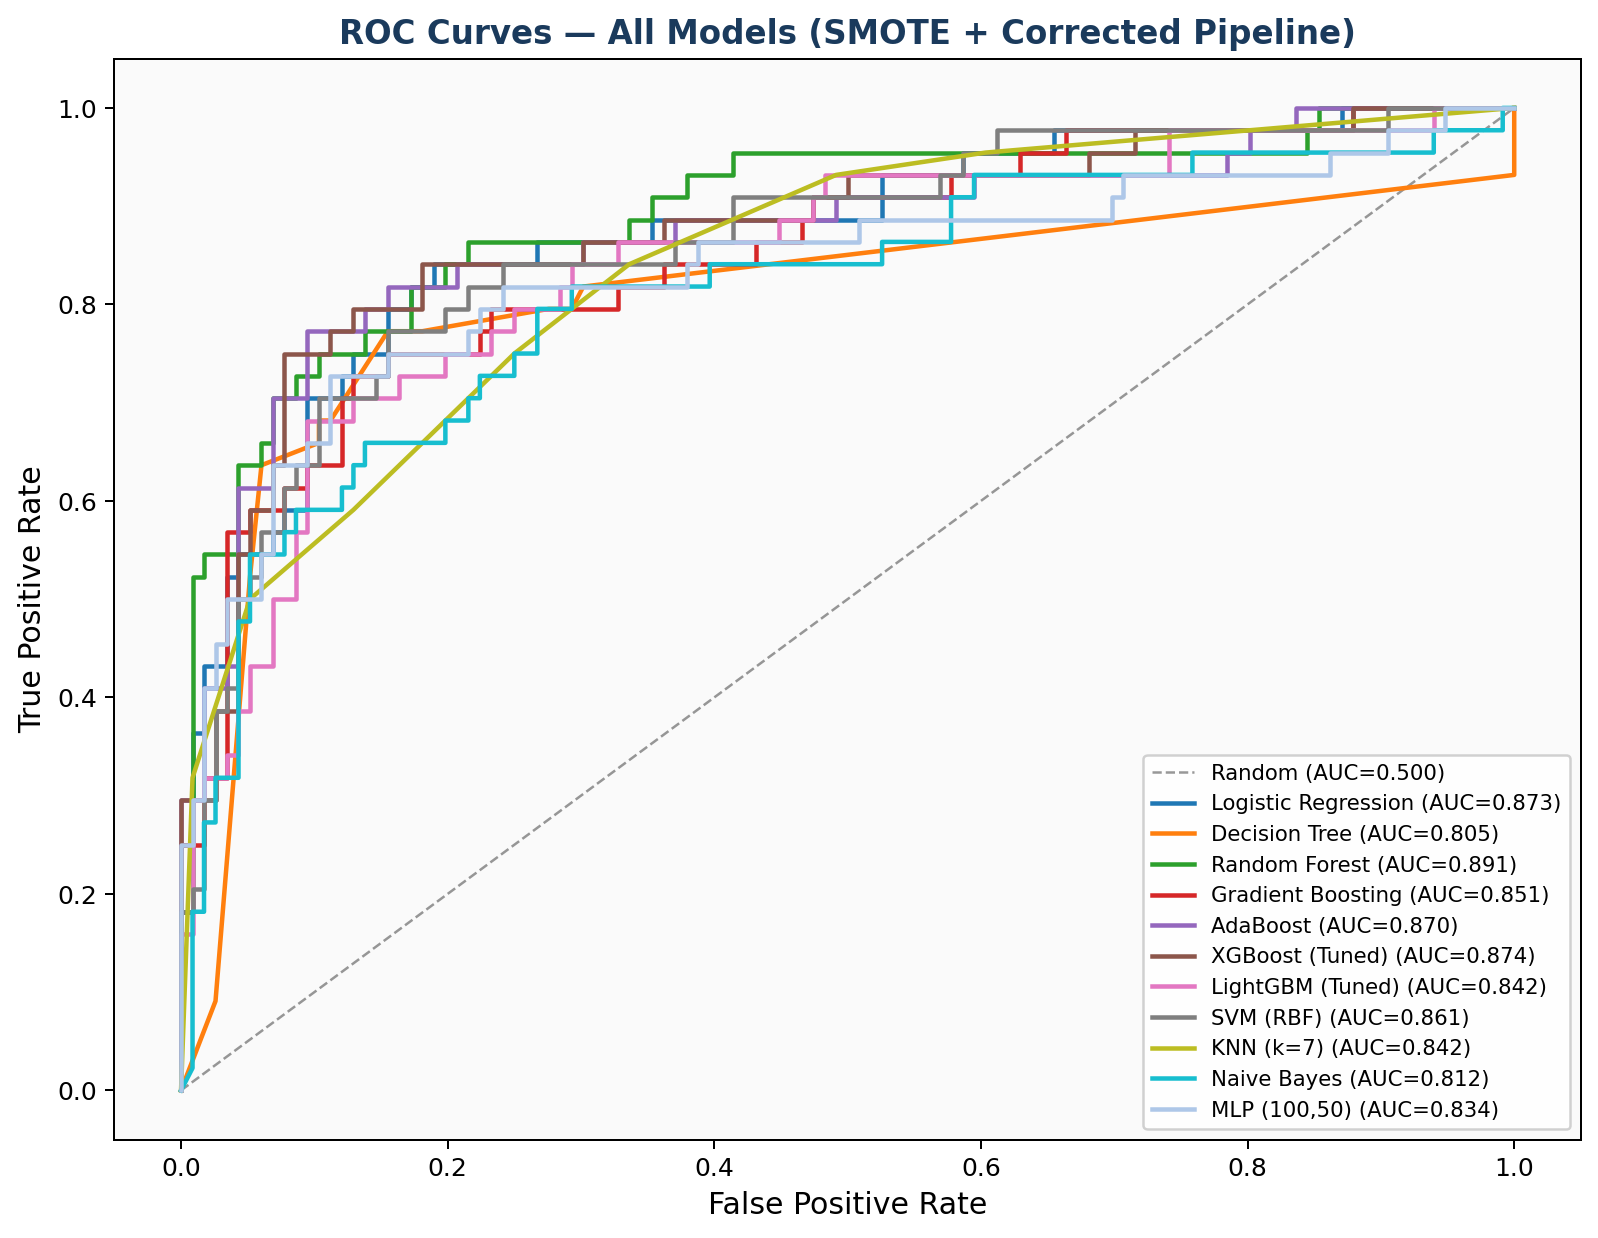
\includegraphics[width=\linewidth]{figures/fig01_roc_single.png}
\caption{ROC curves for all 11 models on the held-out test set ($n=160$).}
\label{fig:roc}
\end{figure}

\begin{figure}[htbp]
\centering
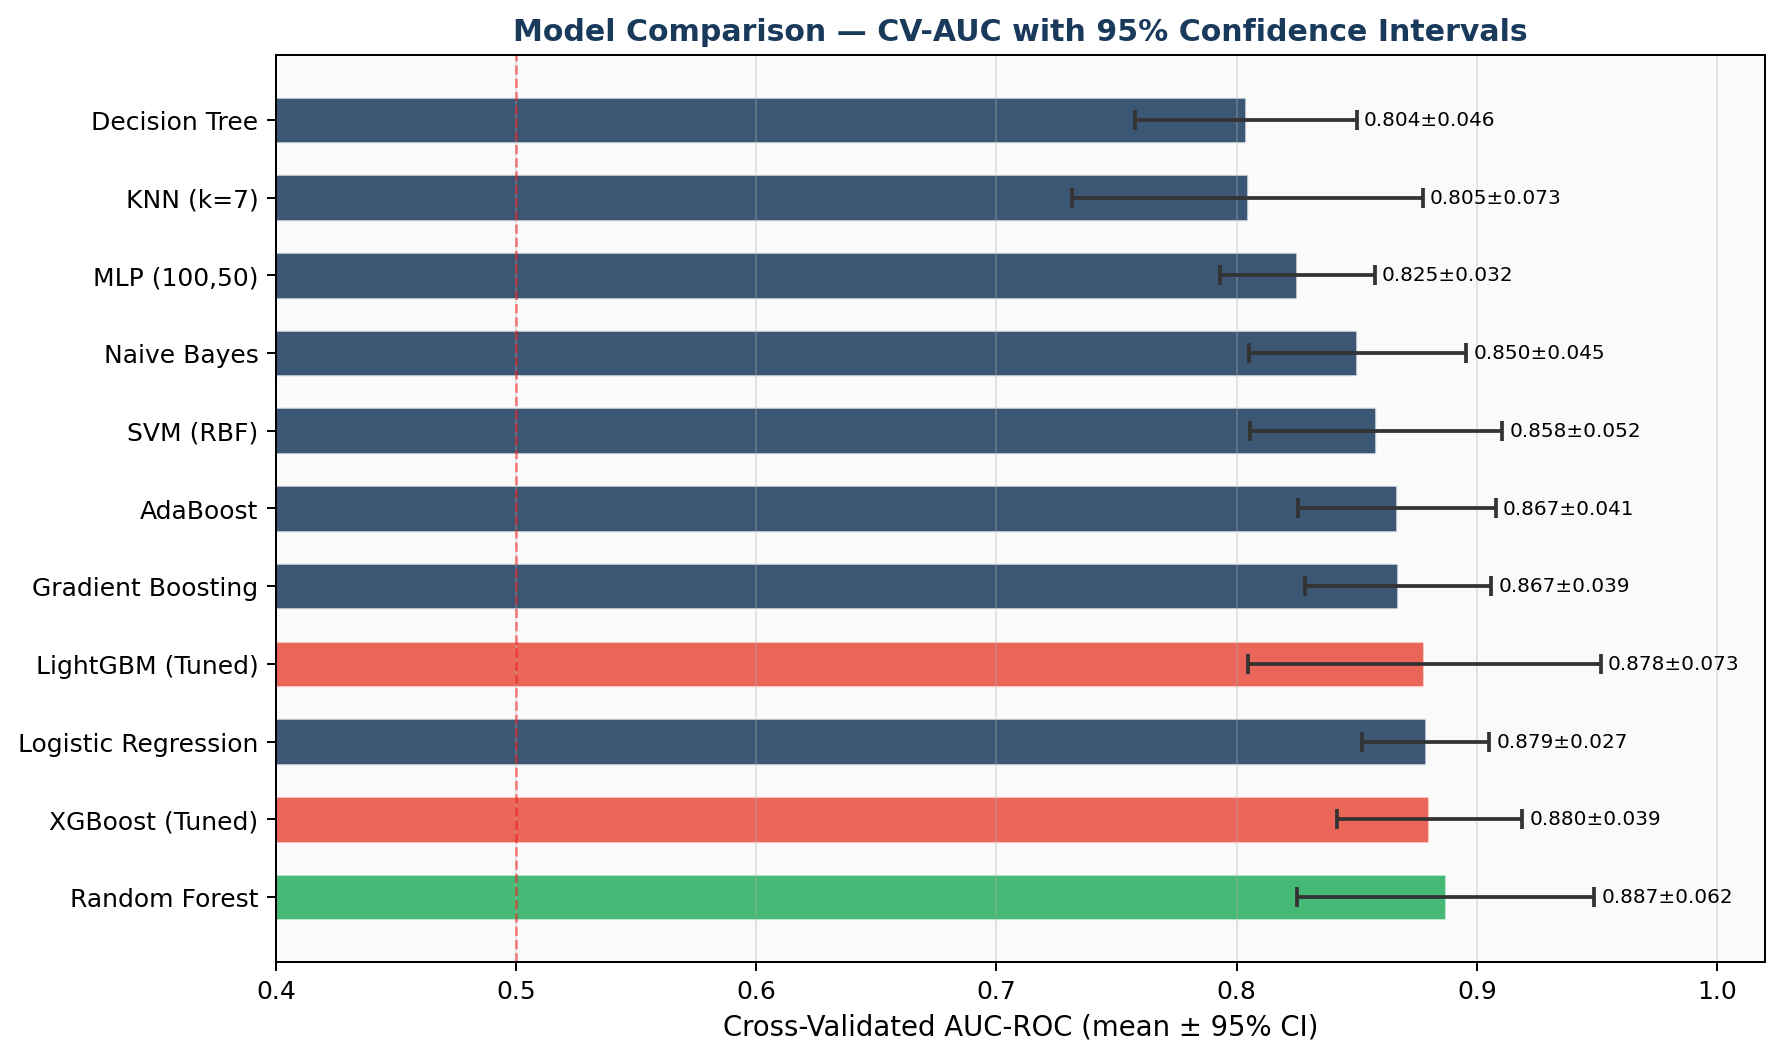
\includegraphics[width=\linewidth]{figures/fig02_cvauc_ci.png}
\caption{Cross-validated AUC-ROC with 95\% confidence intervals for all 11 models, ranked by mean CV-AUC.}
\label{fig:cvauc}
\end{figure}

\begin{figure}[htbp]
\centering
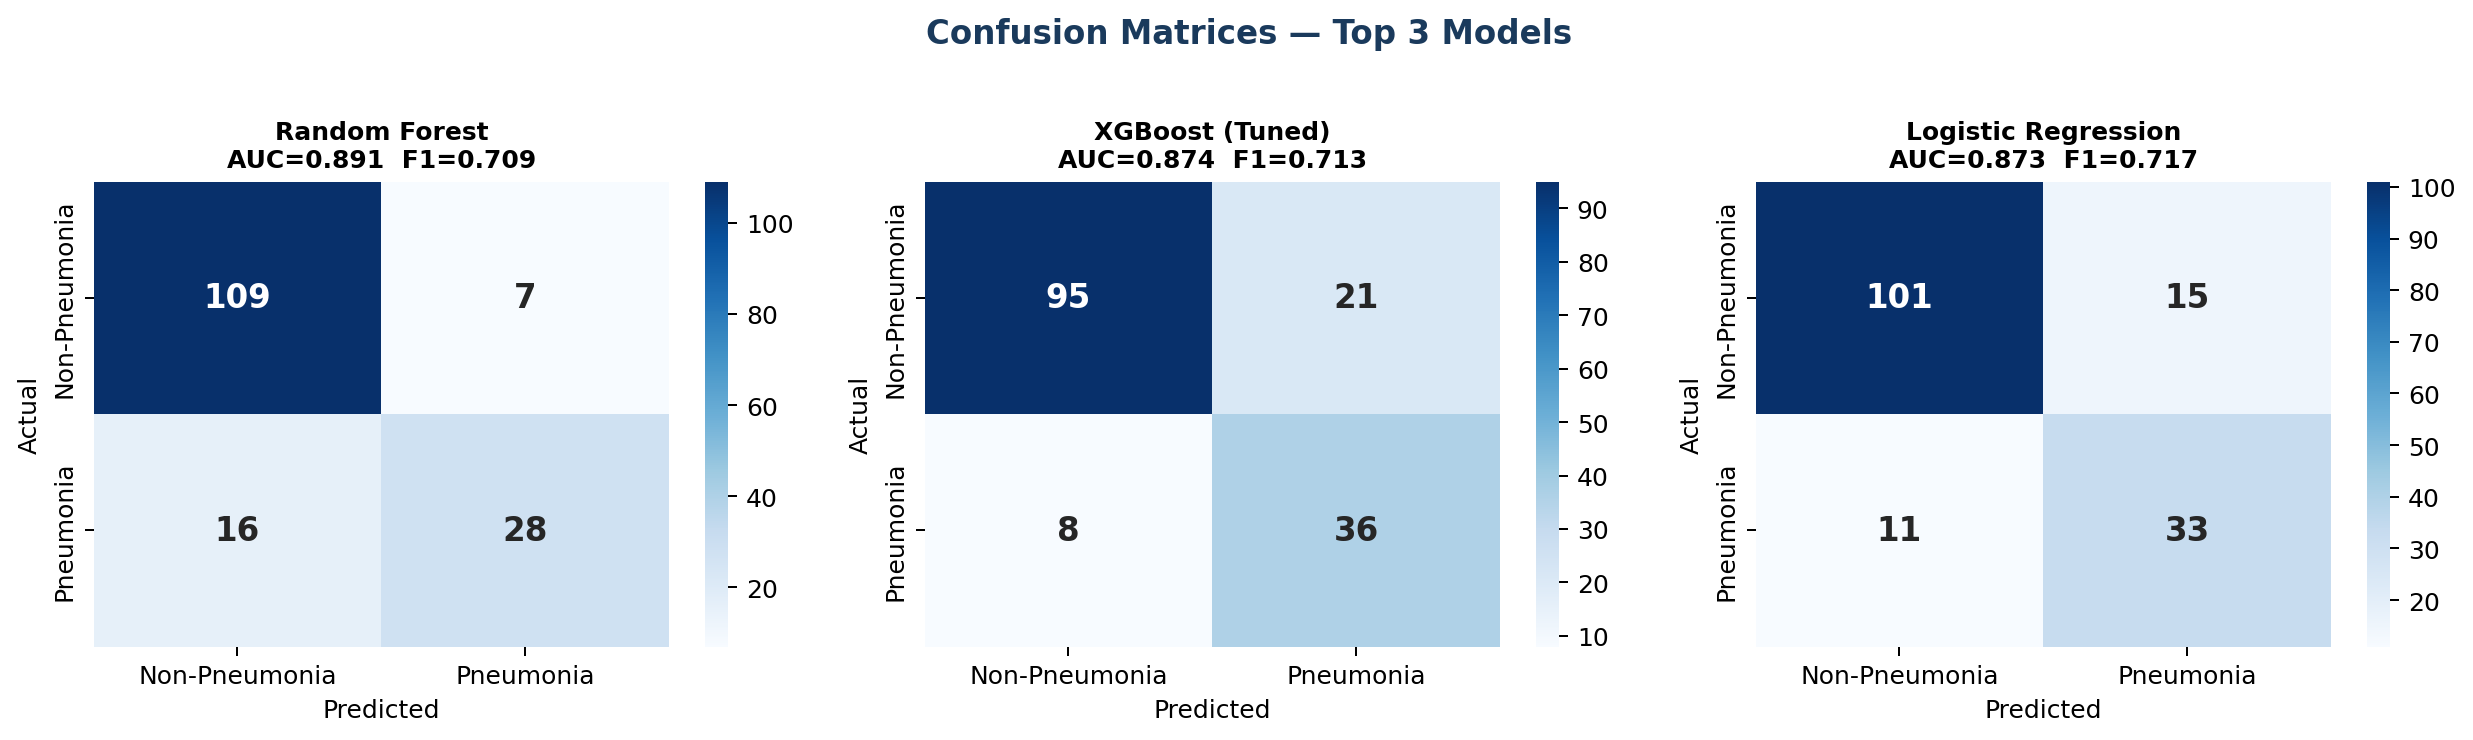
\includegraphics[width=\linewidth]{figures/fig03_confusion_matrices.png}
\caption{Confusion matrices for the top 3 models on the held-out test set ($n=160$).}
\label{fig:confmat}
\end{figure}

Random Forest achieved the best CV-AUC of 0.887 (95\% CI: 0.825--0.949). XGBoost (tuned) achieved the highest test-set Recall of 0.818, most critical for a screening application where false negatives carry clinical risk. Logistic Regression's narrow confidence interval ($\pm$0.027) reflects high cross-fold stability, a clinically desirable property for deployment. The consistent competitiveness of Logistic Regression with ensemble methods suggests primary feature-outcome relationships are approximately linear in the standardized feature space, enabling a transparent paper-and-pencil scoring system.

\subsection{Statistical model comparison: DeLong and McNemar tests}
Table~\ref{tab:delong} presents pairwise DeLong and McNemar test results.

\begin{table}[htbp]
\centering
\caption{Pairwise DeLong (AUC) and McNemar (prediction) statistical tests. NS = not significant.}
\label{tab:delong}
\footnotesize
\begin{tabular}{@{}lccc@{}}
\toprule
Comparison & DeLong $Z$ & $p$ & Result \\
\midrule
RF vs.\ XGBoost & 0.268 & 0.788 & NS \\
RF vs.\ LightGBM & 0.771 & 0.441 & NS \\
RF vs.\ Log.\ Reg. & 0.405 & 0.685 & NS \\
XGBoost vs.\ LightGBM & 0.505 & 0.614 & NS \\
XGBoost vs.\ Log.\ Reg. & 0.133 & 0.894 & NS \\
LightGBM vs.\ Log.\ Reg. & $-0.378$ & 0.706 & NS \\
\bottomrule
\end{tabular}
\end{table}

All pairwise DeLong and McNemar tests are non-significant (all $p > 0.05$), indicating that the AUC differences observed between the top four models (RF: 0.891, XGB: 0.874, LGB: 0.854, LR: 0.873) are within sampling variability on this test set. This finding has an important practical implication: model selection between these top candidates should be guided by secondary criteria -- calibration quality, interpretability, computational requirements, and deployment context -- rather than AUC alone.

\begin{figure}[htbp]
\centering
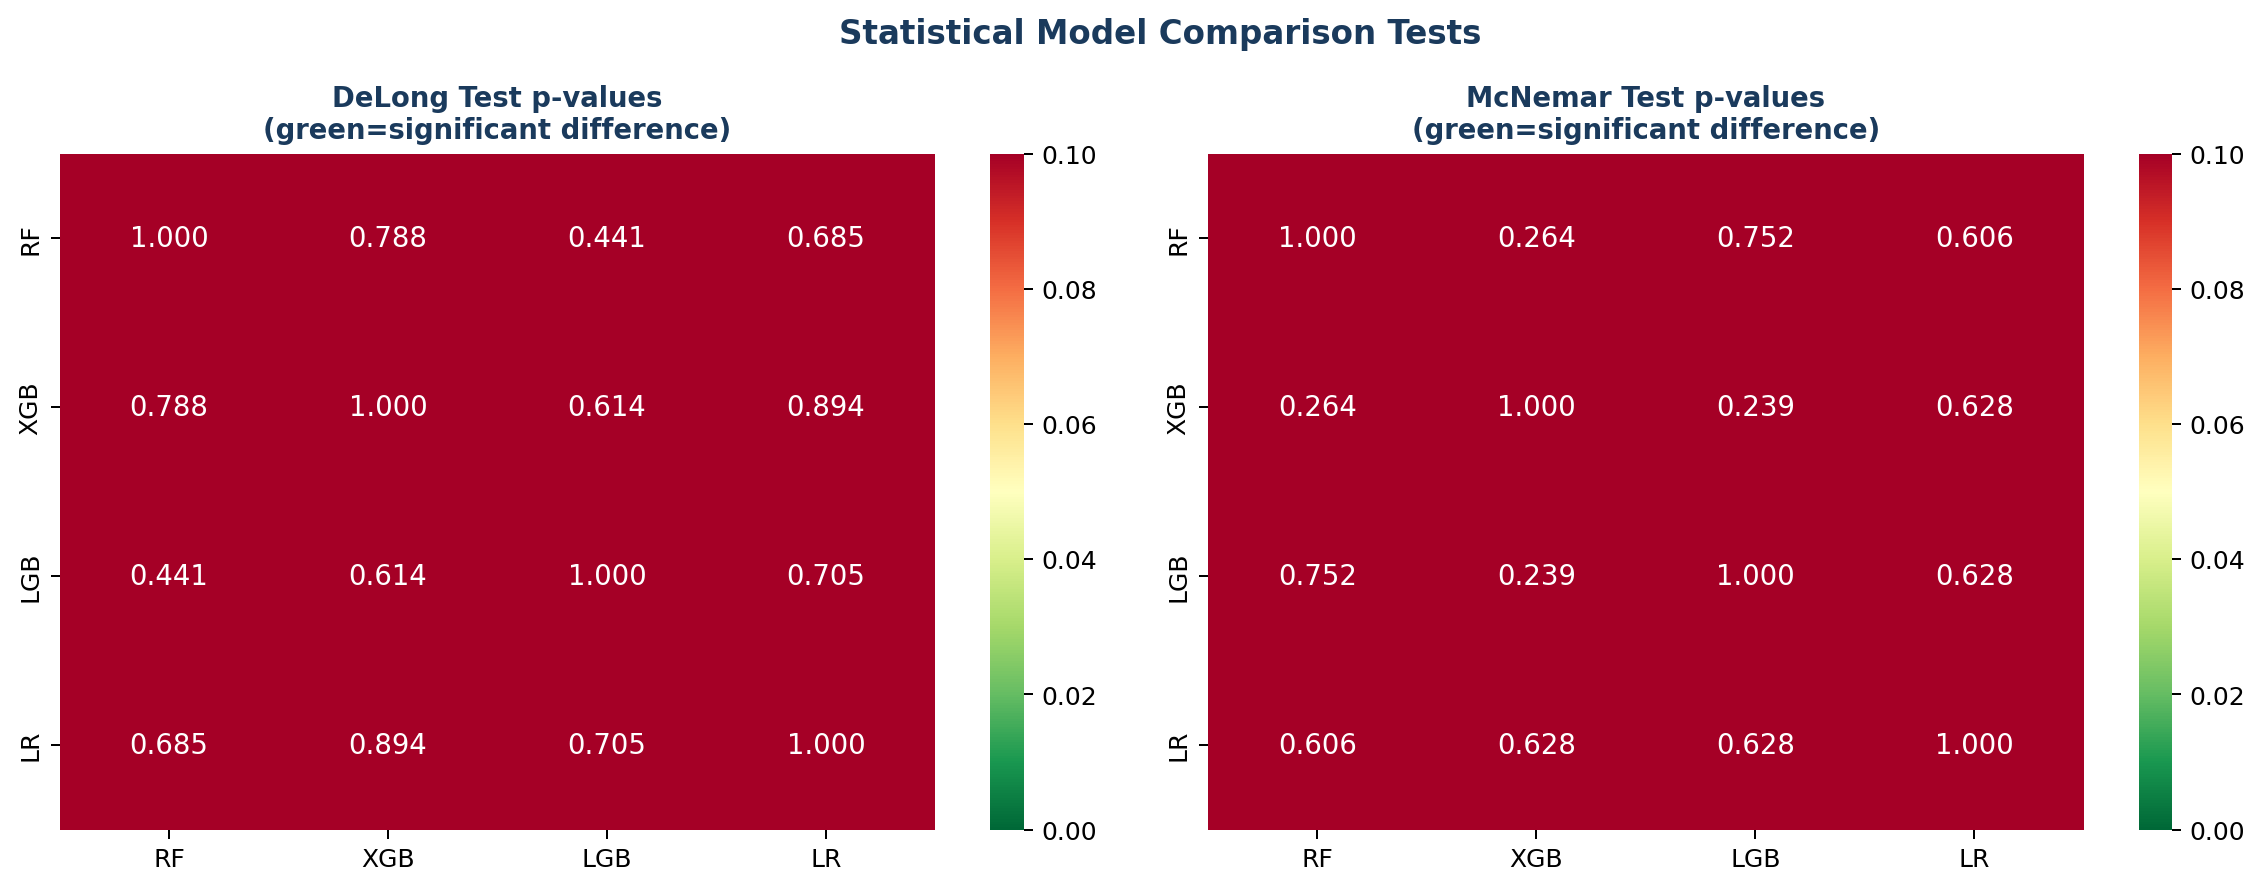
\includegraphics[width=\linewidth]{figures/fig04_delong_mcnemar.png}
\caption{DeLong and McNemar test $p$-value heatmaps across the top-4 models (RF, XGB, LGB, LR). Lower values (green) indicate significant differences.}
\label{fig:delongheat}
\end{figure}

\subsection{Probability calibration analysis}
Table~\ref{tab:calibration} and Fig.~\ref{fig:calibration} present calibration results.

\begin{table}[htbp]
\centering
\caption{Probability calibration analysis. $\downarrow$ = lower is better.}
\label{tab:calibration}
\footnotesize
\begin{tabular}{@{}lccl@{}}
\toprule
Model & Brier$\downarrow$ & ECE$\downarrow$ & Quality \\
\midrule
Random Forest & \textbf{0.1092} & \textbf{0.0519} & Best \\
Logistic Regression & 0.1246 & 0.0806 & Good \\
XGBoost (Tuned) & 0.1317 & 0.1249 & Fair \\
LightGBM (Tuned) & 0.1370 & 0.1427 & Fair \\
\bottomrule
\end{tabular}
\end{table}

\begin{figure}[htbp]
\centering
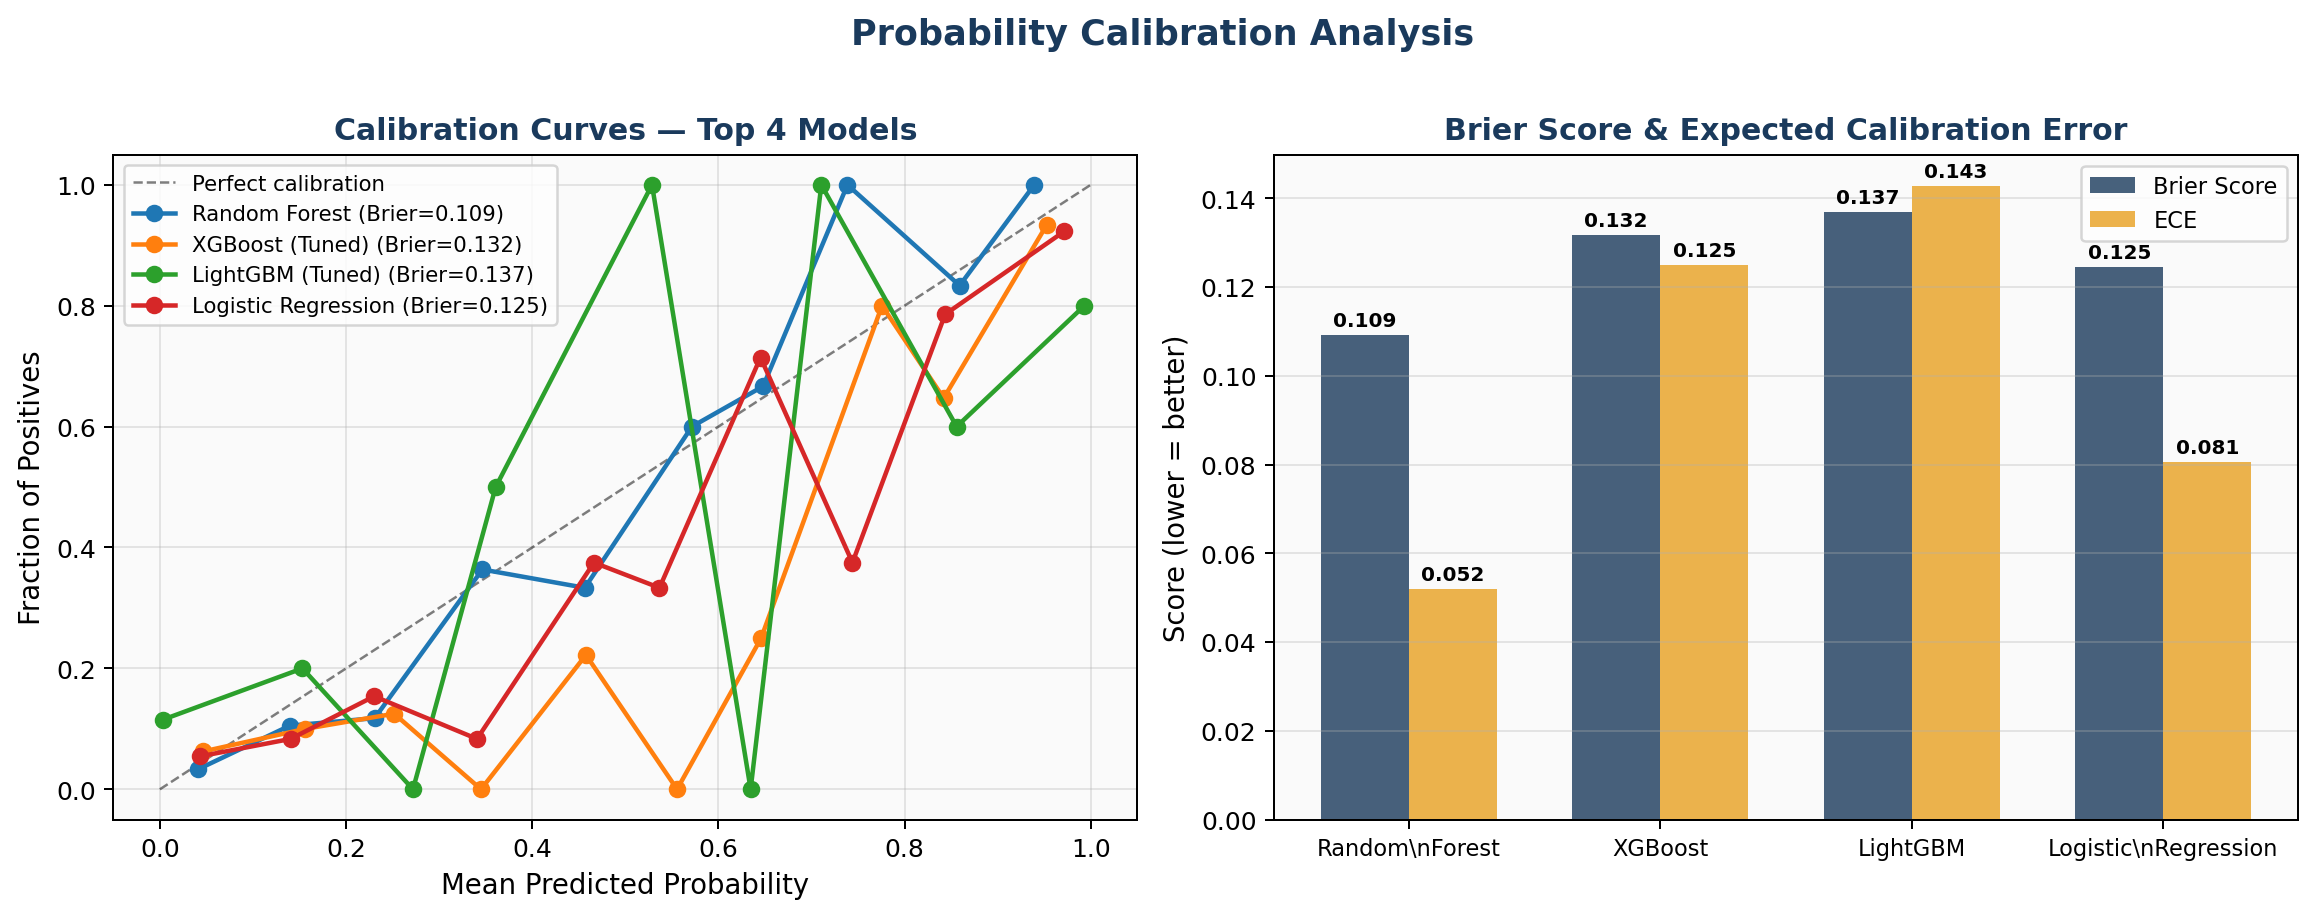
\includegraphics[width=\linewidth]{figures/fig05_calibration.png}
\caption{Calibration curves (left) and Brier Score / ECE bar chart (right) for the top 4 models.}
\label{fig:calibration}
\end{figure}

Random Forest is the best-calibrated model, producing probability estimates most closely aligned with observed outcome frequencies. XGBoost and LightGBM show higher ECE values, indicating systematic overconfidence at high predicted probabilities, a common characteristic of gradient boosting models trained on imbalanced data. The CPSS thresholds ($P<0.35$, $0.35$--$0.65$, $P>0.65$) were derived using Random Forest probabilities to ensure well-calibrated boundary conditions.

\subsection{Decision Curve Analysis}
Fig.~\ref{fig:dca} demonstrates that all four ML models provide positive net benefit over the treat-none strategy across the clinically relevant threshold range of approximately 0.10--0.60. At thresholds below 0.15, all models outperform the treat-all strategy, indicating that model-based triage reduces unnecessary referrals without sacrificing sensitivity.

\begin{figure}[htbp]
\centering
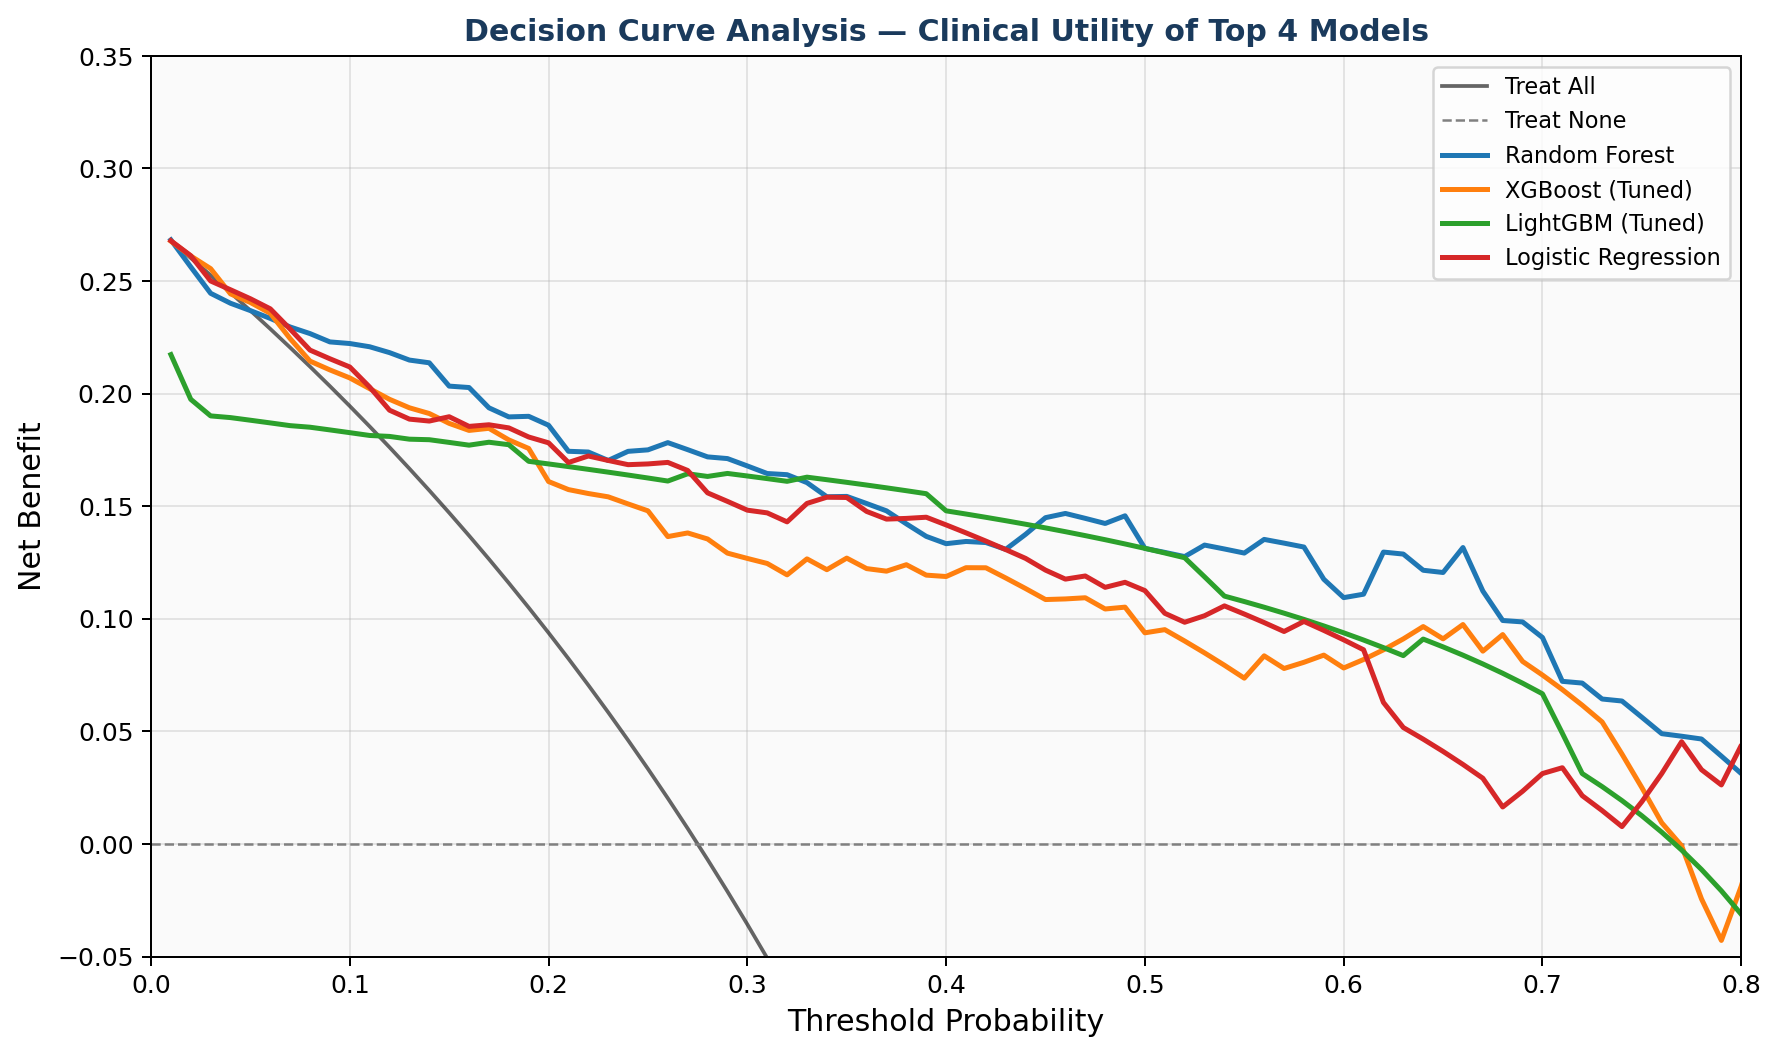
\includegraphics[width=\linewidth]{figures/fig06_dca.png}
\caption{Decision Curve Analysis for the top 4 models. Net benefit across threshold probabilities, compared to treat-all and treat-none strategies.}
\label{fig:dca}
\end{figure}

\subsection{Feature importance and SHAP analysis}
Fig.~\ref{fig:featimp} shows the top 15 feature importances, and Fig.~\ref{fig:shap} the SHAP summary plot.

\begin{figure}[htbp]
\centering
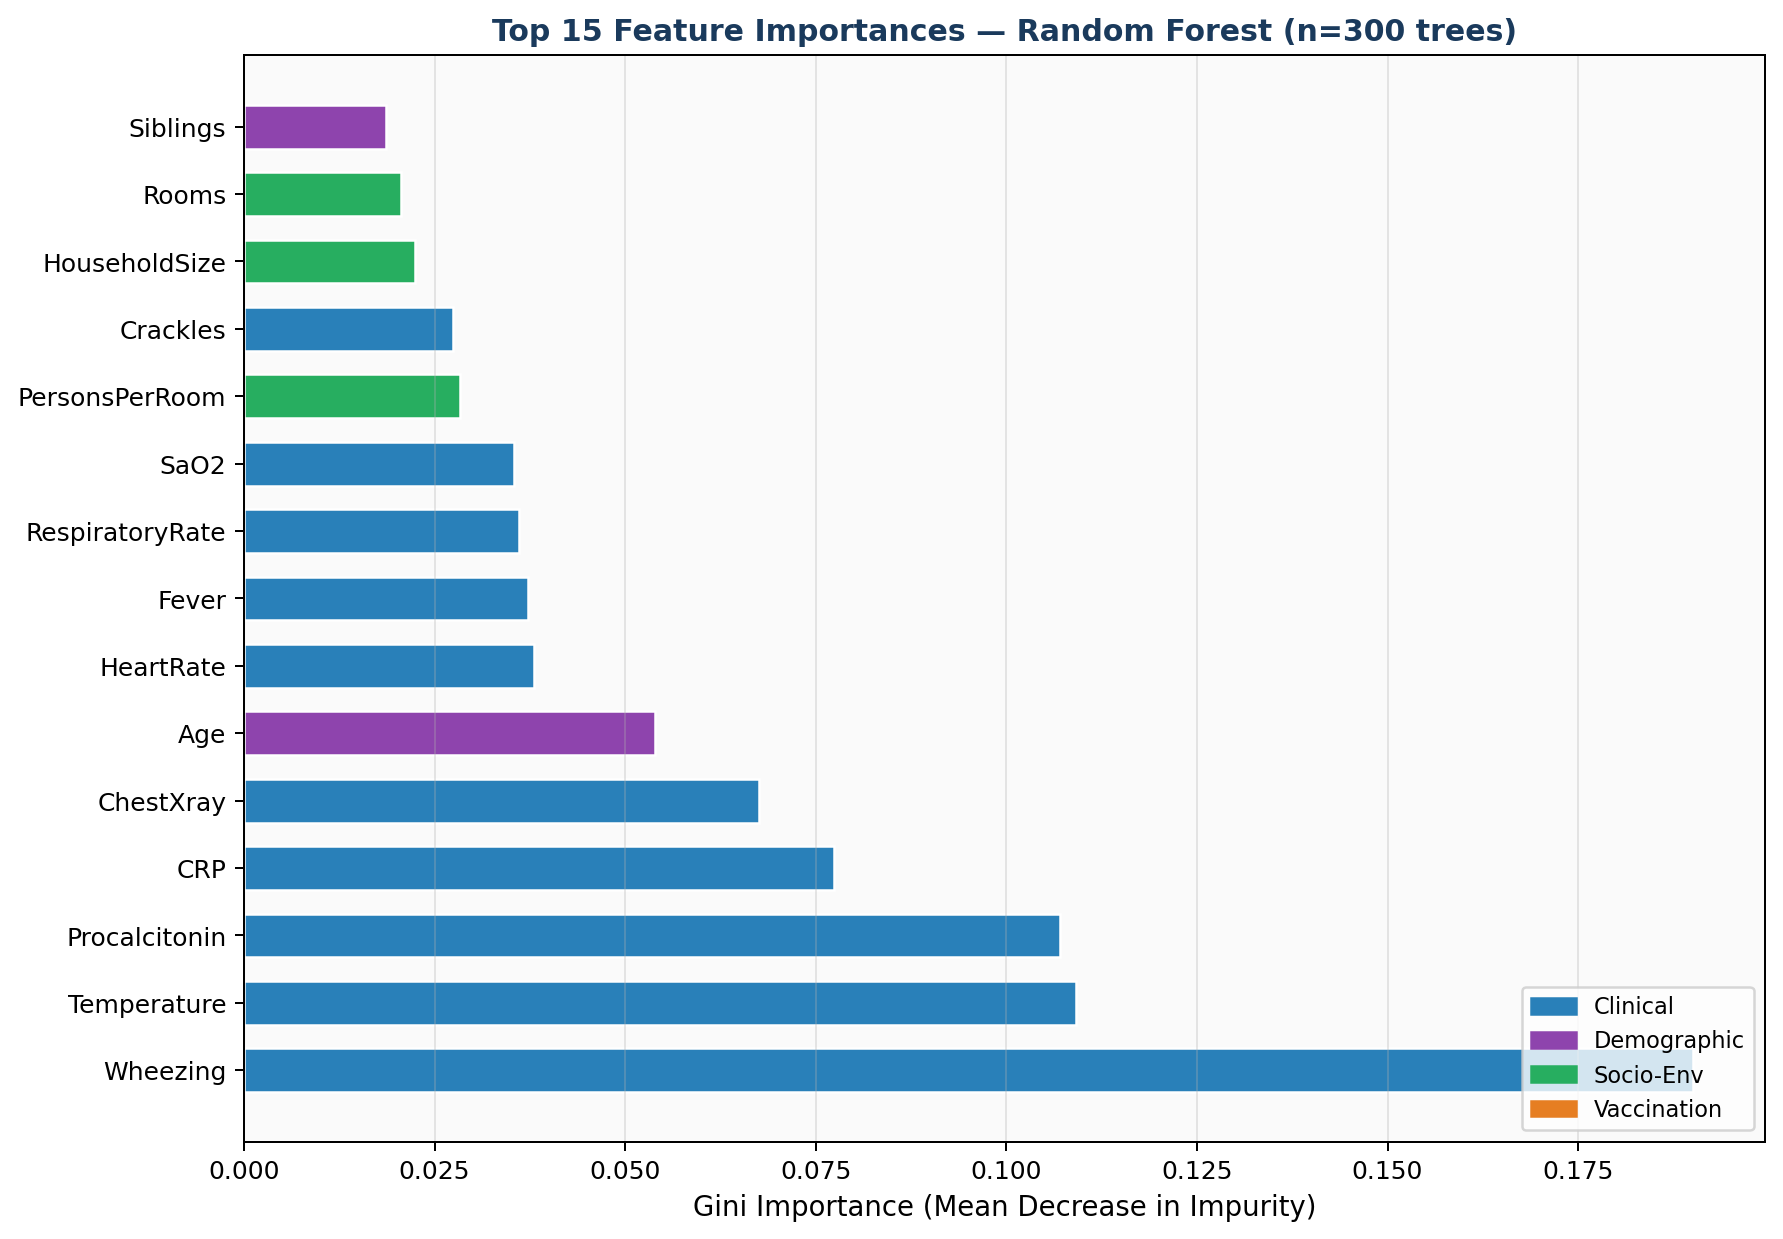
\includegraphics[width=\linewidth]{figures/fig07_feature_importance.png}
\caption{Top 15 feature importances (Random Forest, 300 trees), colour-coded by category.}
\label{fig:featimp}
\end{figure}

\begin{figure}[htbp]
\centering
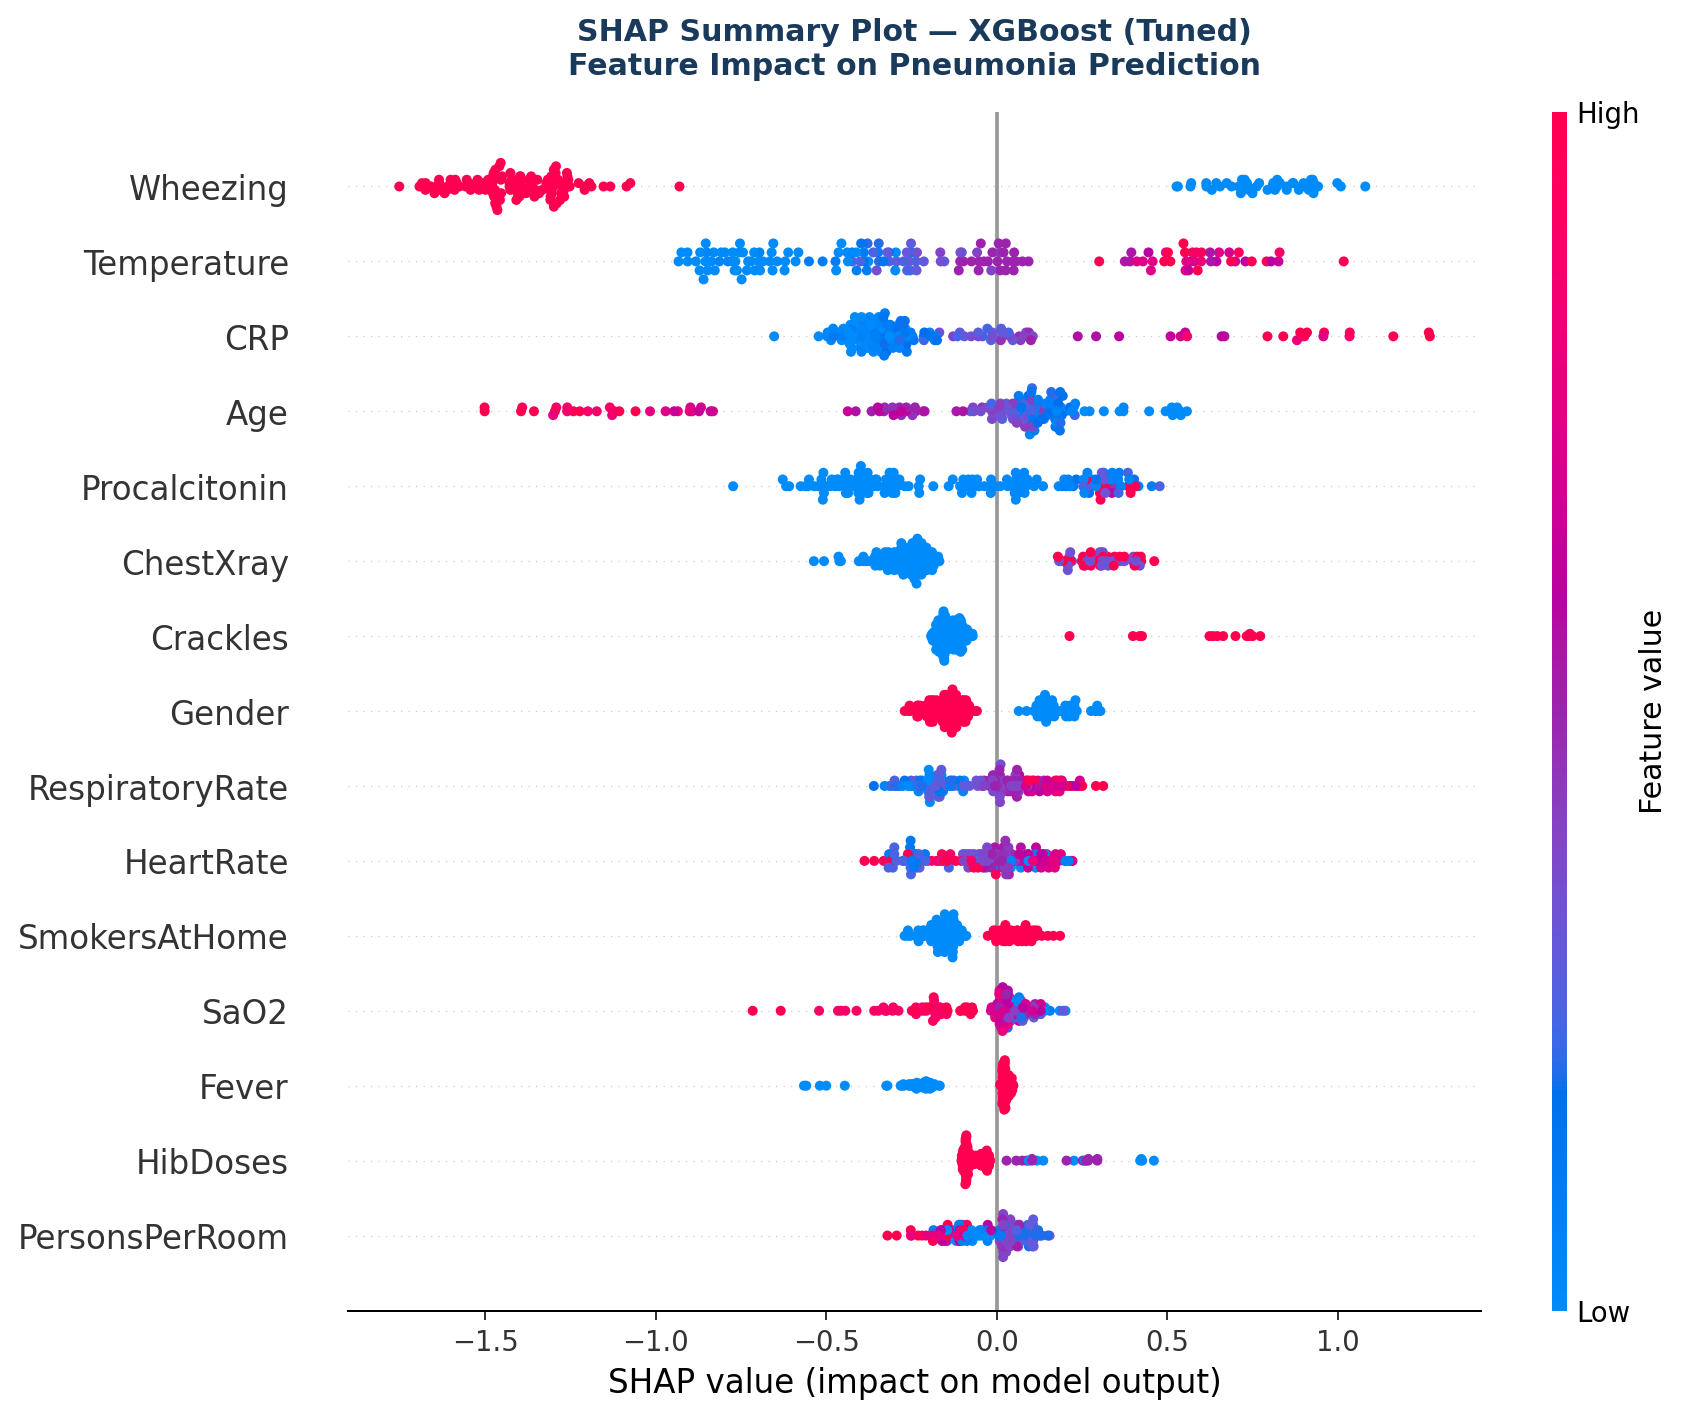
\includegraphics[width=\linewidth]{figures/fig08_shap_summary.png}
\caption{SHAP summary plot for the tuned XGBoost model. Red~=~high feature value, blue~=~low. X-axis~=~impact on pneumonia prediction probability.}
\label{fig:shap}
\end{figure}

Wheezing dominates individual feature importance (Gini~=~0.190, $\chi^2=226.7$, $p<0.001$), reflecting strong discrimination between pneumonia and other acute respiratory conditions. At the category level, clinical features contribute 59.1\%, demographic 13.1\%, socio-environmental 9.4\%, and vaccination 7.0\% of total predictive importance. SHAP dependence analysis (Fig.~\ref{fig:shapdep}) reveals important nonlinear patterns: wheezing presence shifts SHAP contribution sharply positive; PersonsPerRoom shows a positive monotonic SHAP trend at higher values, providing patient-level confirmation of the crowding hypothesis; temperature shows a positive association above approximately 38.5\textdegree C; and Procalcitonin shows strong positive SHAP values above 0.5~ng/mL.

\begin{figure}[htbp]
\centering
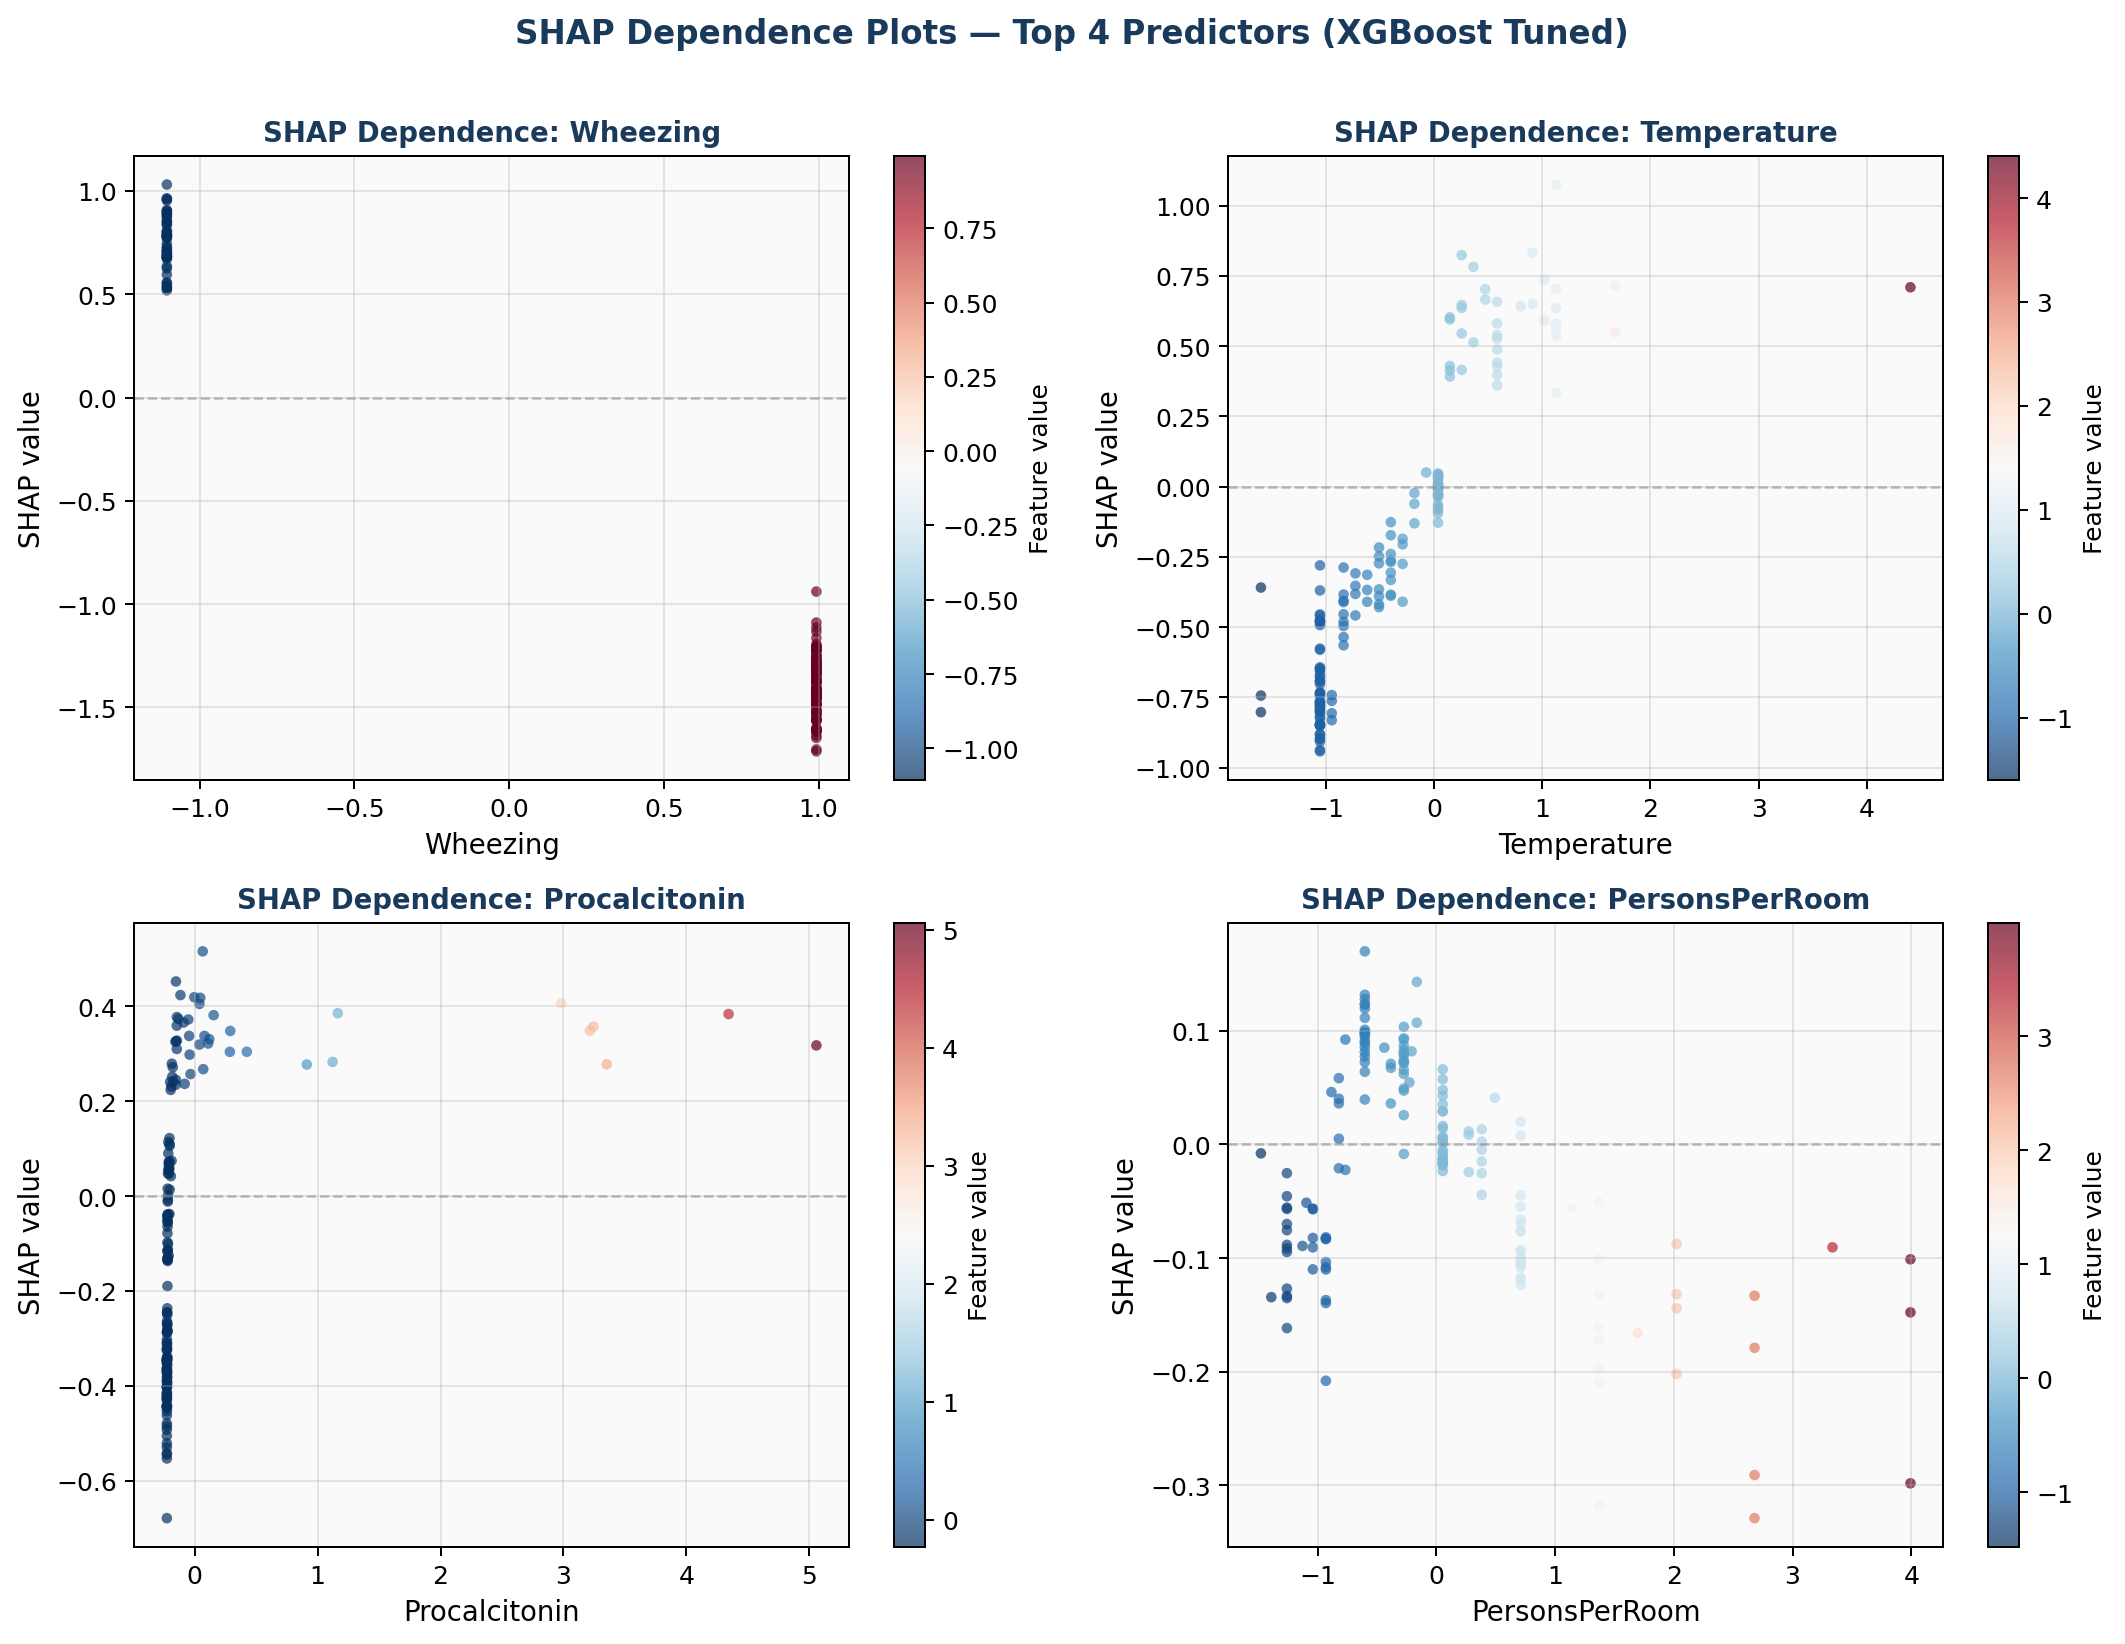
\includegraphics[width=\linewidth]{figures/fig09_shap_dependence.png}
\caption{SHAP dependence plots for the top 4 features: wheezing, temperature, procalcitonin, persons-per-room.}
\label{fig:shapdep}
\end{figure}

Individual waterfall plots (Fig.~\ref{fig:waterfall}) enable clinicians to understand exactly which features drive each prediction for representative low-, moderate-, and high-risk patients.

\begin{figure}[htbp]
\centering
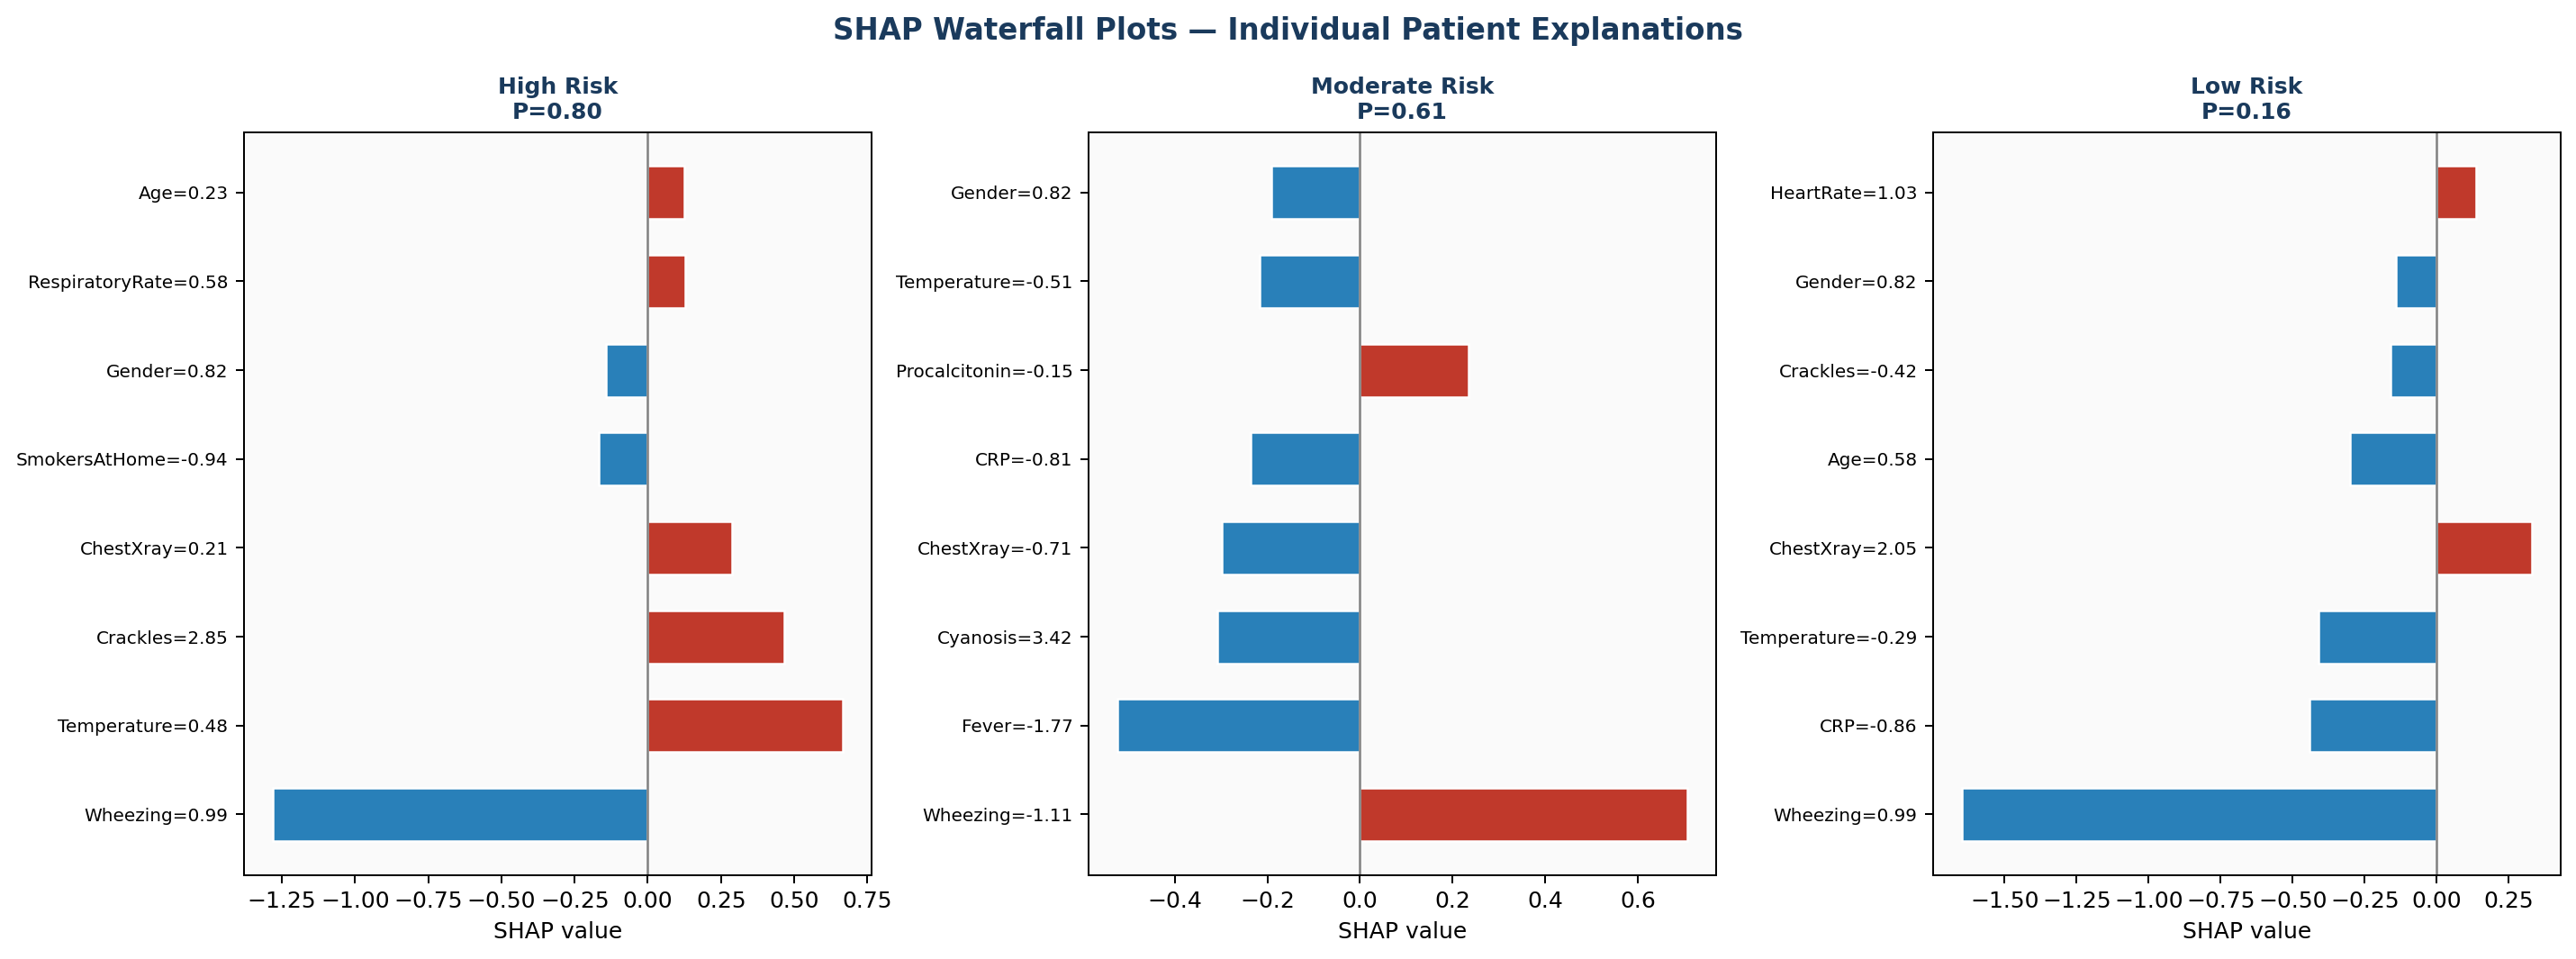
\includegraphics[width=\linewidth]{figures/fig10_shap_waterfall.png}
\caption{SHAP waterfall plots for individual representative patients: high-, moderate-, and low-risk cases (tuned XGBoost).}
\label{fig:waterfall}
\end{figure}

\subsection{CERS optimization analysis}
Fig.~\ref{fig:cers} compares expert-defined and data-driven CERS weights.

\begin{figure}[htbp]
\centering
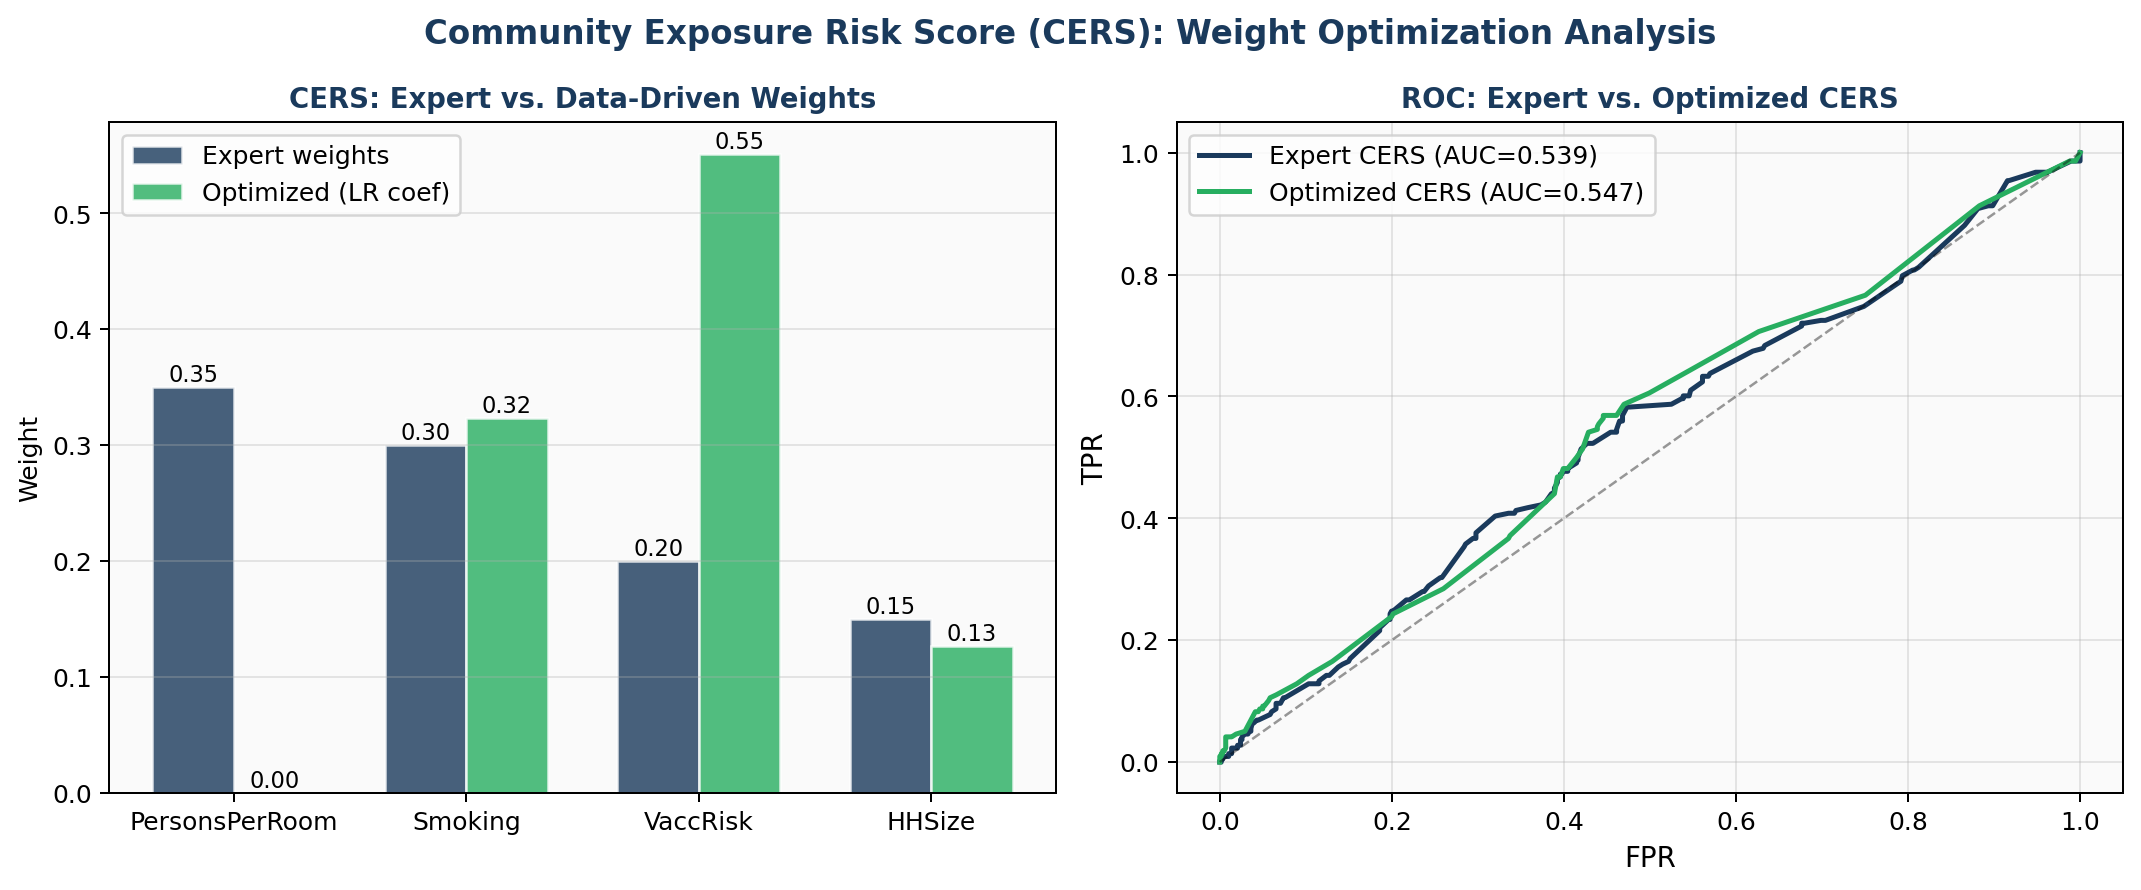
\includegraphics[width=\linewidth]{figures/fig11_cers_optimization.png}
\caption{CERS weight optimization: expert vs.\ data-driven (logistic regression) weights (left), and ROC comparison of both CERS variants (right).}
\label{fig:cers}
\end{figure}

Data-driven CERS optimization assigned the dominant weight to VaccinationRisk (0.551), followed by Smoking (0.323) and HHSize (0.126), with PersonsPerRoom receiving near-zero weight (0.000). This contrasts with the expert-defined weights and reveals that -- in this cohort where 87.6\% are fully vaccinated -- vaccination status carries substantially higher individual discriminatory power than crowding, whose chi-square $p$-value was non-significant ($p=0.166$).

\subsection{Vaccination prevalence and crowding analysis}
Fig.~\ref{fig:vacc} and Fig.~\ref{fig:crowd} illustrate the population-level associations. The vaccination--pneumonia association follows a clear monotonic dose-response gradient (fully vaccinated: 25.2\%, partially: 40.2\%, unvaccinated: 57.1\%; $\chi^2=11.1$, $p<0.001$), consistent with immunological theory and prior epidemiological evidence \cite{ref8,ref9,ref10}.

\begin{figure}[htbp]
\centering
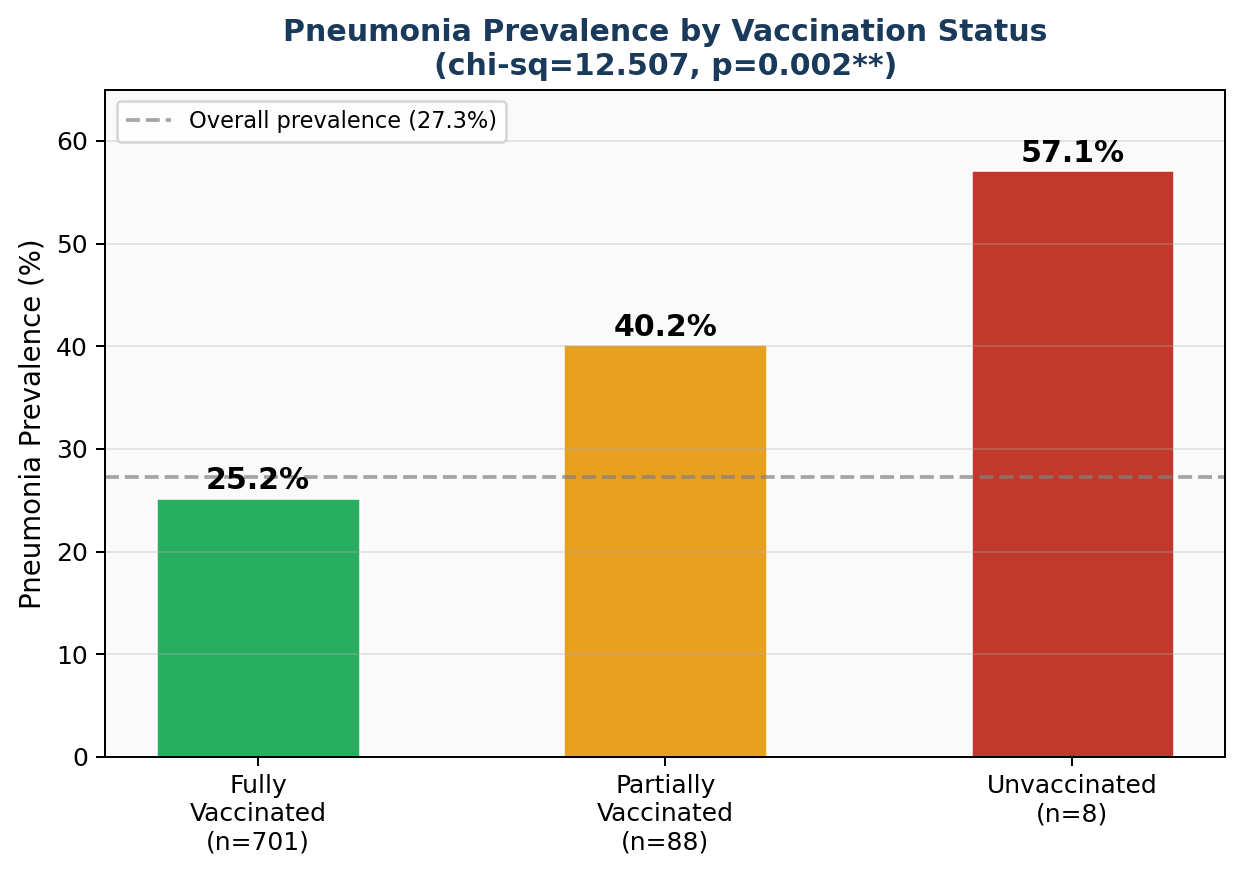
\includegraphics[width=0.85\linewidth]{figures/fig12_vacc_prevalence.png}
\caption{Pneumonia prevalence by vaccination status ($\chi^2=11.1$, $p<0.001$), showing a step-wise 25.2\%$\rightarrow$40.2\%$\rightarrow$57.1\% gradient.}
\label{fig:vacc}
\end{figure}

\begin{figure}[htbp]
\centering
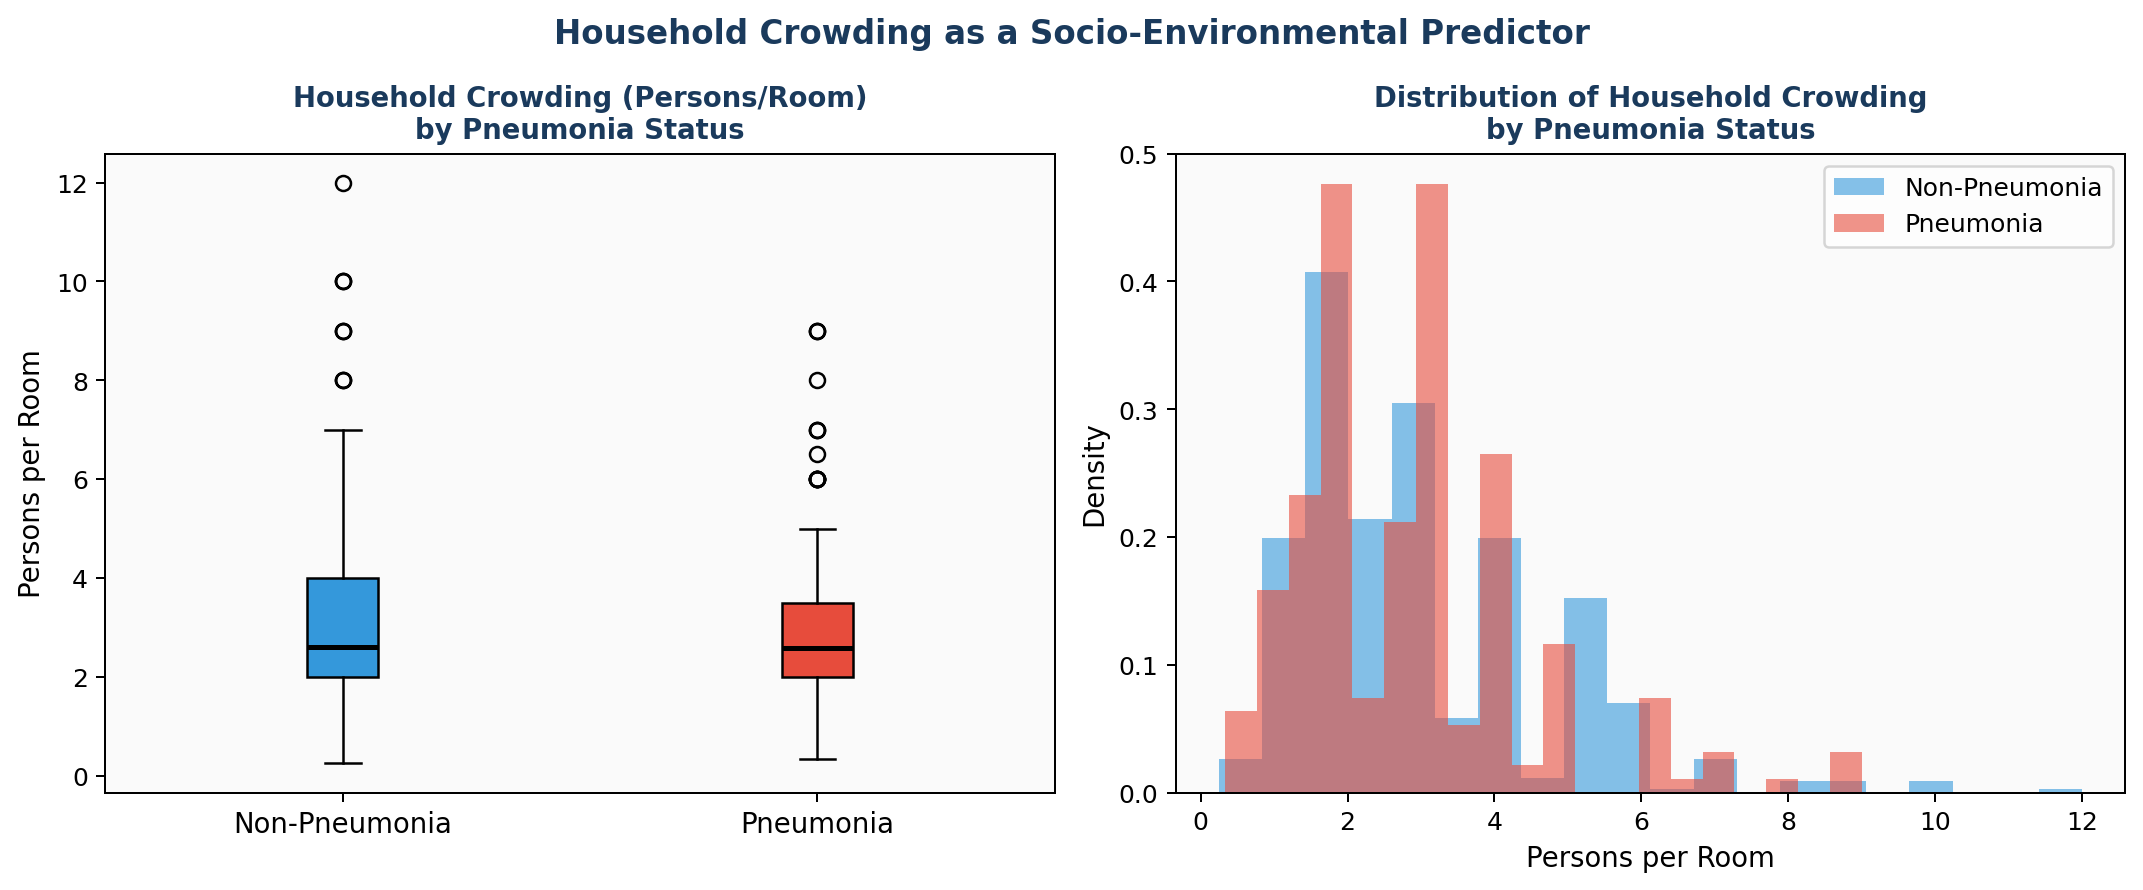
\includegraphics[width=\linewidth]{figures/fig13_crowding.png}
\caption{Household crowding (persons per room) distribution by pneumonia diagnosis.}
\label{fig:crowd}
\end{figure}

\subsection{Fairness and subgroup analysis}
Table~\ref{tab:fairness} and Fig.~\ref{fig:fairness} present fairness results across six demographic subgroups.

\begin{table}[htbp]
\centering
\caption{Fairness analysis: Random Forest performance across demographic subgroups.}
\label{tab:fairness}
\footnotesize
\begin{tabular}{@{}lcccc@{}}
\toprule
Subgroup & $n$ & AUC & Recall \\
\midrule
Male & 102 & 0.918 & 0.656 \\
Female & 58 & 0.846 & 0.583 \\
Infant ($\leq$12 mo.) & 57 & 0.853 & 0.571 \\
Older child ($>$12 mo.) & 103 & 0.890 & 0.696 \\
Fully vaccinated & 139 & 0.881 & 0.611 \\
Not fully vaccinated & 21 & 0.962 & 0.750 \\
\bottomrule
\end{tabular}
\end{table}

\begin{figure}[htbp]
\centering
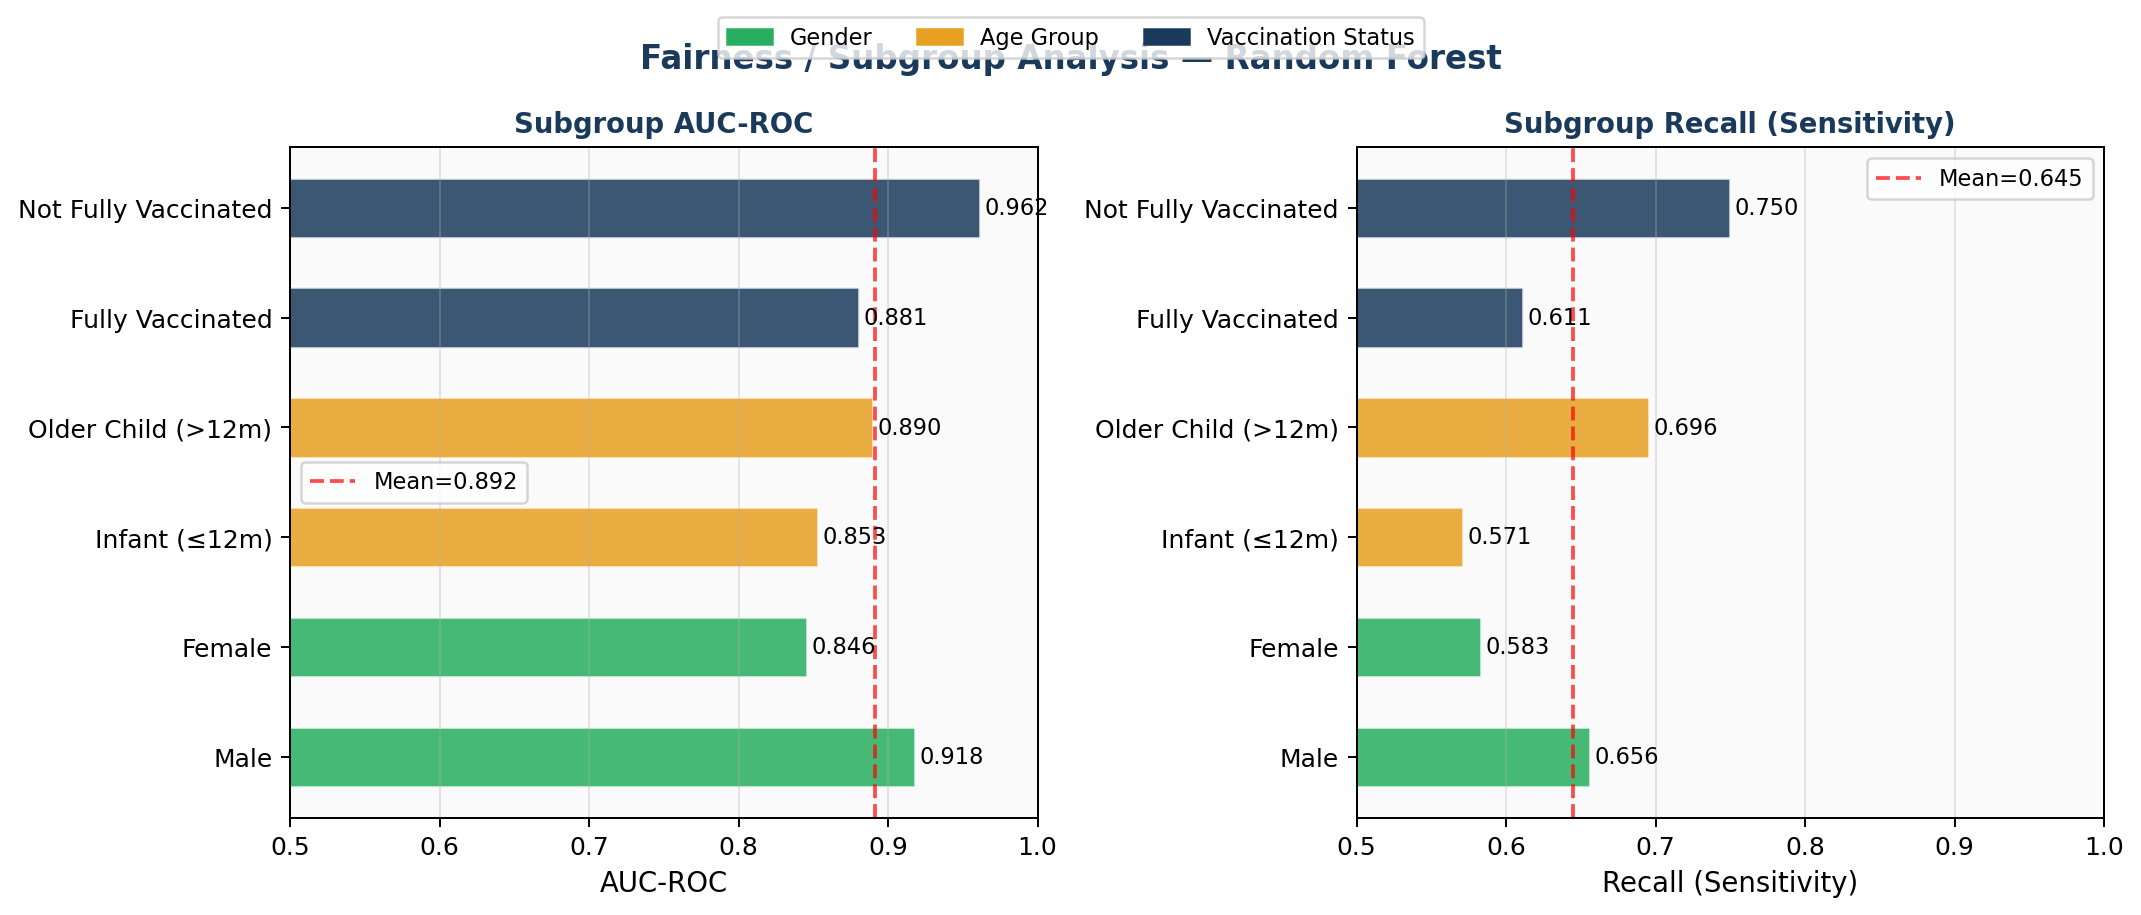
\includegraphics[width=\linewidth]{figures/fig14_fairness.png}
\caption{Subgroup AUC-ROC (left) and Recall (right) across gender, age, and vaccination status subgroups.}
\label{fig:fairness}
\end{figure}

AUC ranges from 0.846 (Female) to 0.962 (Not Fully Vaccinated) across subgroups, without catastrophic performance collapse in any group. The higher AUC for males likely reflects sample size disparity rather than a genuine biological difference. Older children show higher recall than infants, consistent with more pronounced clinical signs facilitating earlier and more accurate identification. No subgroup shows AUC below 0.84, indicating consistent model reliability across the demographic spectrum evaluated.

\subsection{Sensitivity analysis}
Fig.~\ref{fig:sensitivity} confirms that reported results are not artifacts of a fortuitous random split. Random Forest achieved mean AUC~=~$0.887\pm0.021$ and XGBoost mean AUC~=~$0.875\pm0.022$ across ten seeds.

\begin{figure}[htbp]
\centering
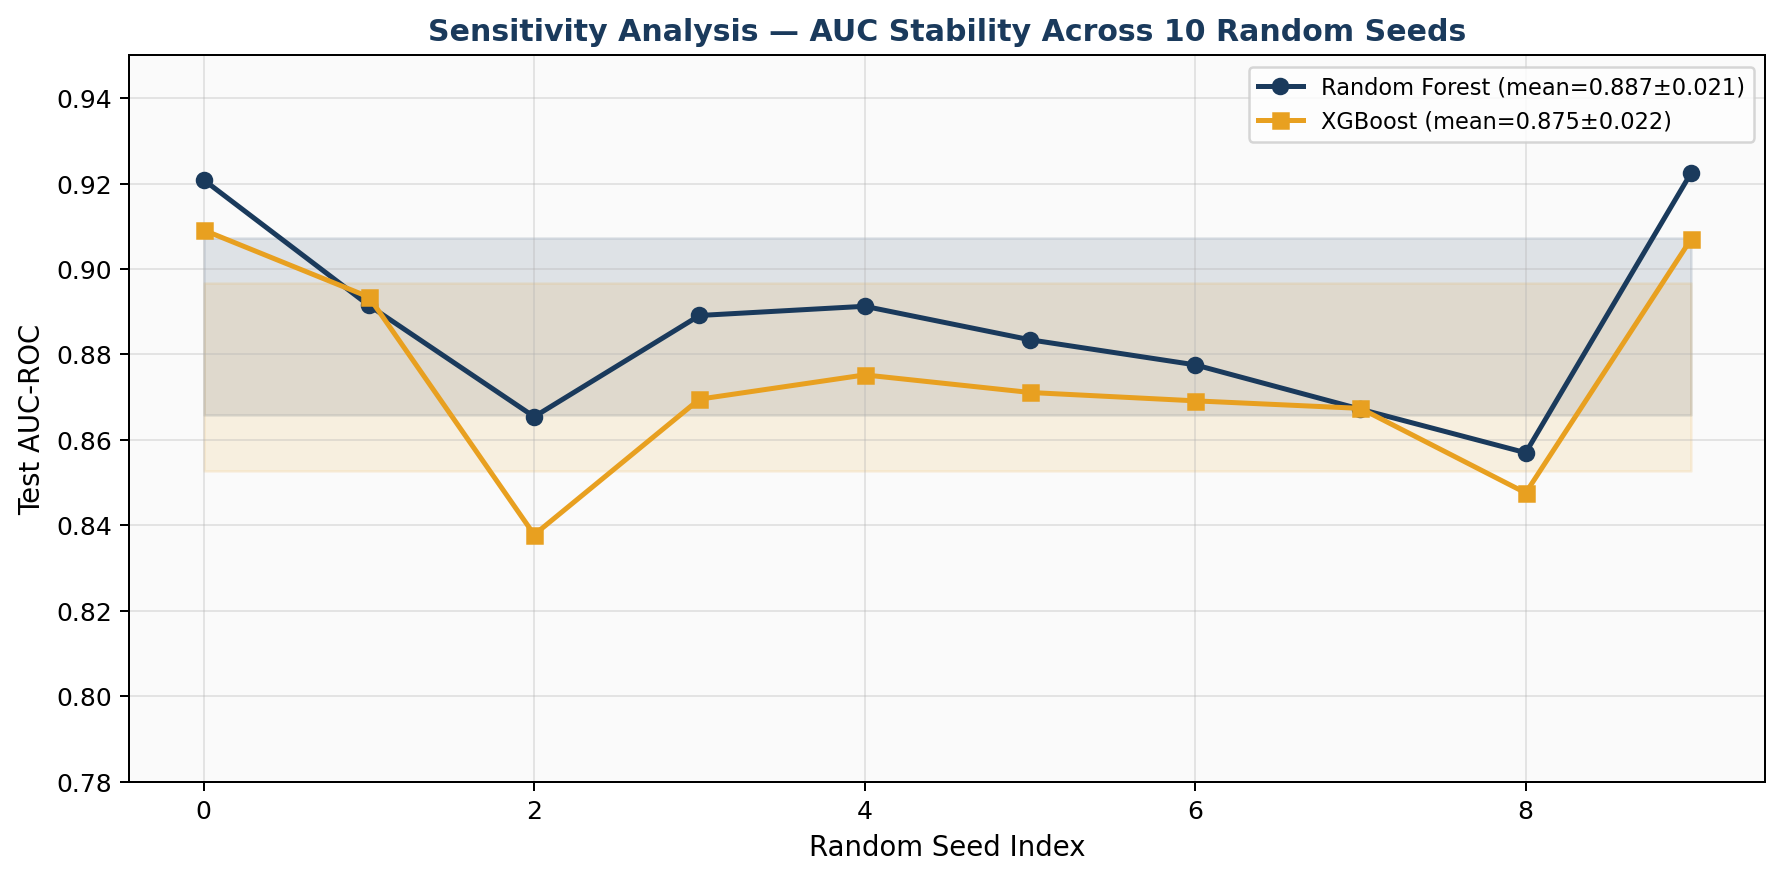
\includegraphics[width=\linewidth]{figures/fig15_sensitivity.png}
\caption{AUC stability across 10 random seeds for Random Forest and XGBoost. Shaded bands~=~$\pm$1 std.\ deviation.}
\label{fig:sensitivity}
\end{figure}

\subsection{Clinical Decision Framework and CPSS}
The CAEPPF Clinical Decision Framework (Fig.~\ref{fig:framework}) operationalizes the ML pipeline into a CHW-deployable workflow. The Community Pneumonia Screening Score (CPSS), derived from Logistic Regression coefficients, enables probability estimation without computational infrastructure:
\begin{equation}
\begin{split}
\text{CPSS} = {}& 2\times\text{Wheezing} + 1.5\times\text{Fever} \\
& + 1\times\text{Crowding} + 1\times\text{VaccRisk} \\
& + 0.5\times\text{Smoking}
\end{split}
\end{equation}

Scores of 0--2 indicate Low Risk (routine monitoring and caregiver education), 3--4 indicate Moderate Risk (early primary care referral within 24--48~h), and $\geq$5 indicate High Risk (immediate hospital referral). SHAP-based explanations accompany each prediction, identifying whether the dominant risk driver is clinical, socio-environmental, or vaccination-related.

\begin{figure}[htbp]
\centering
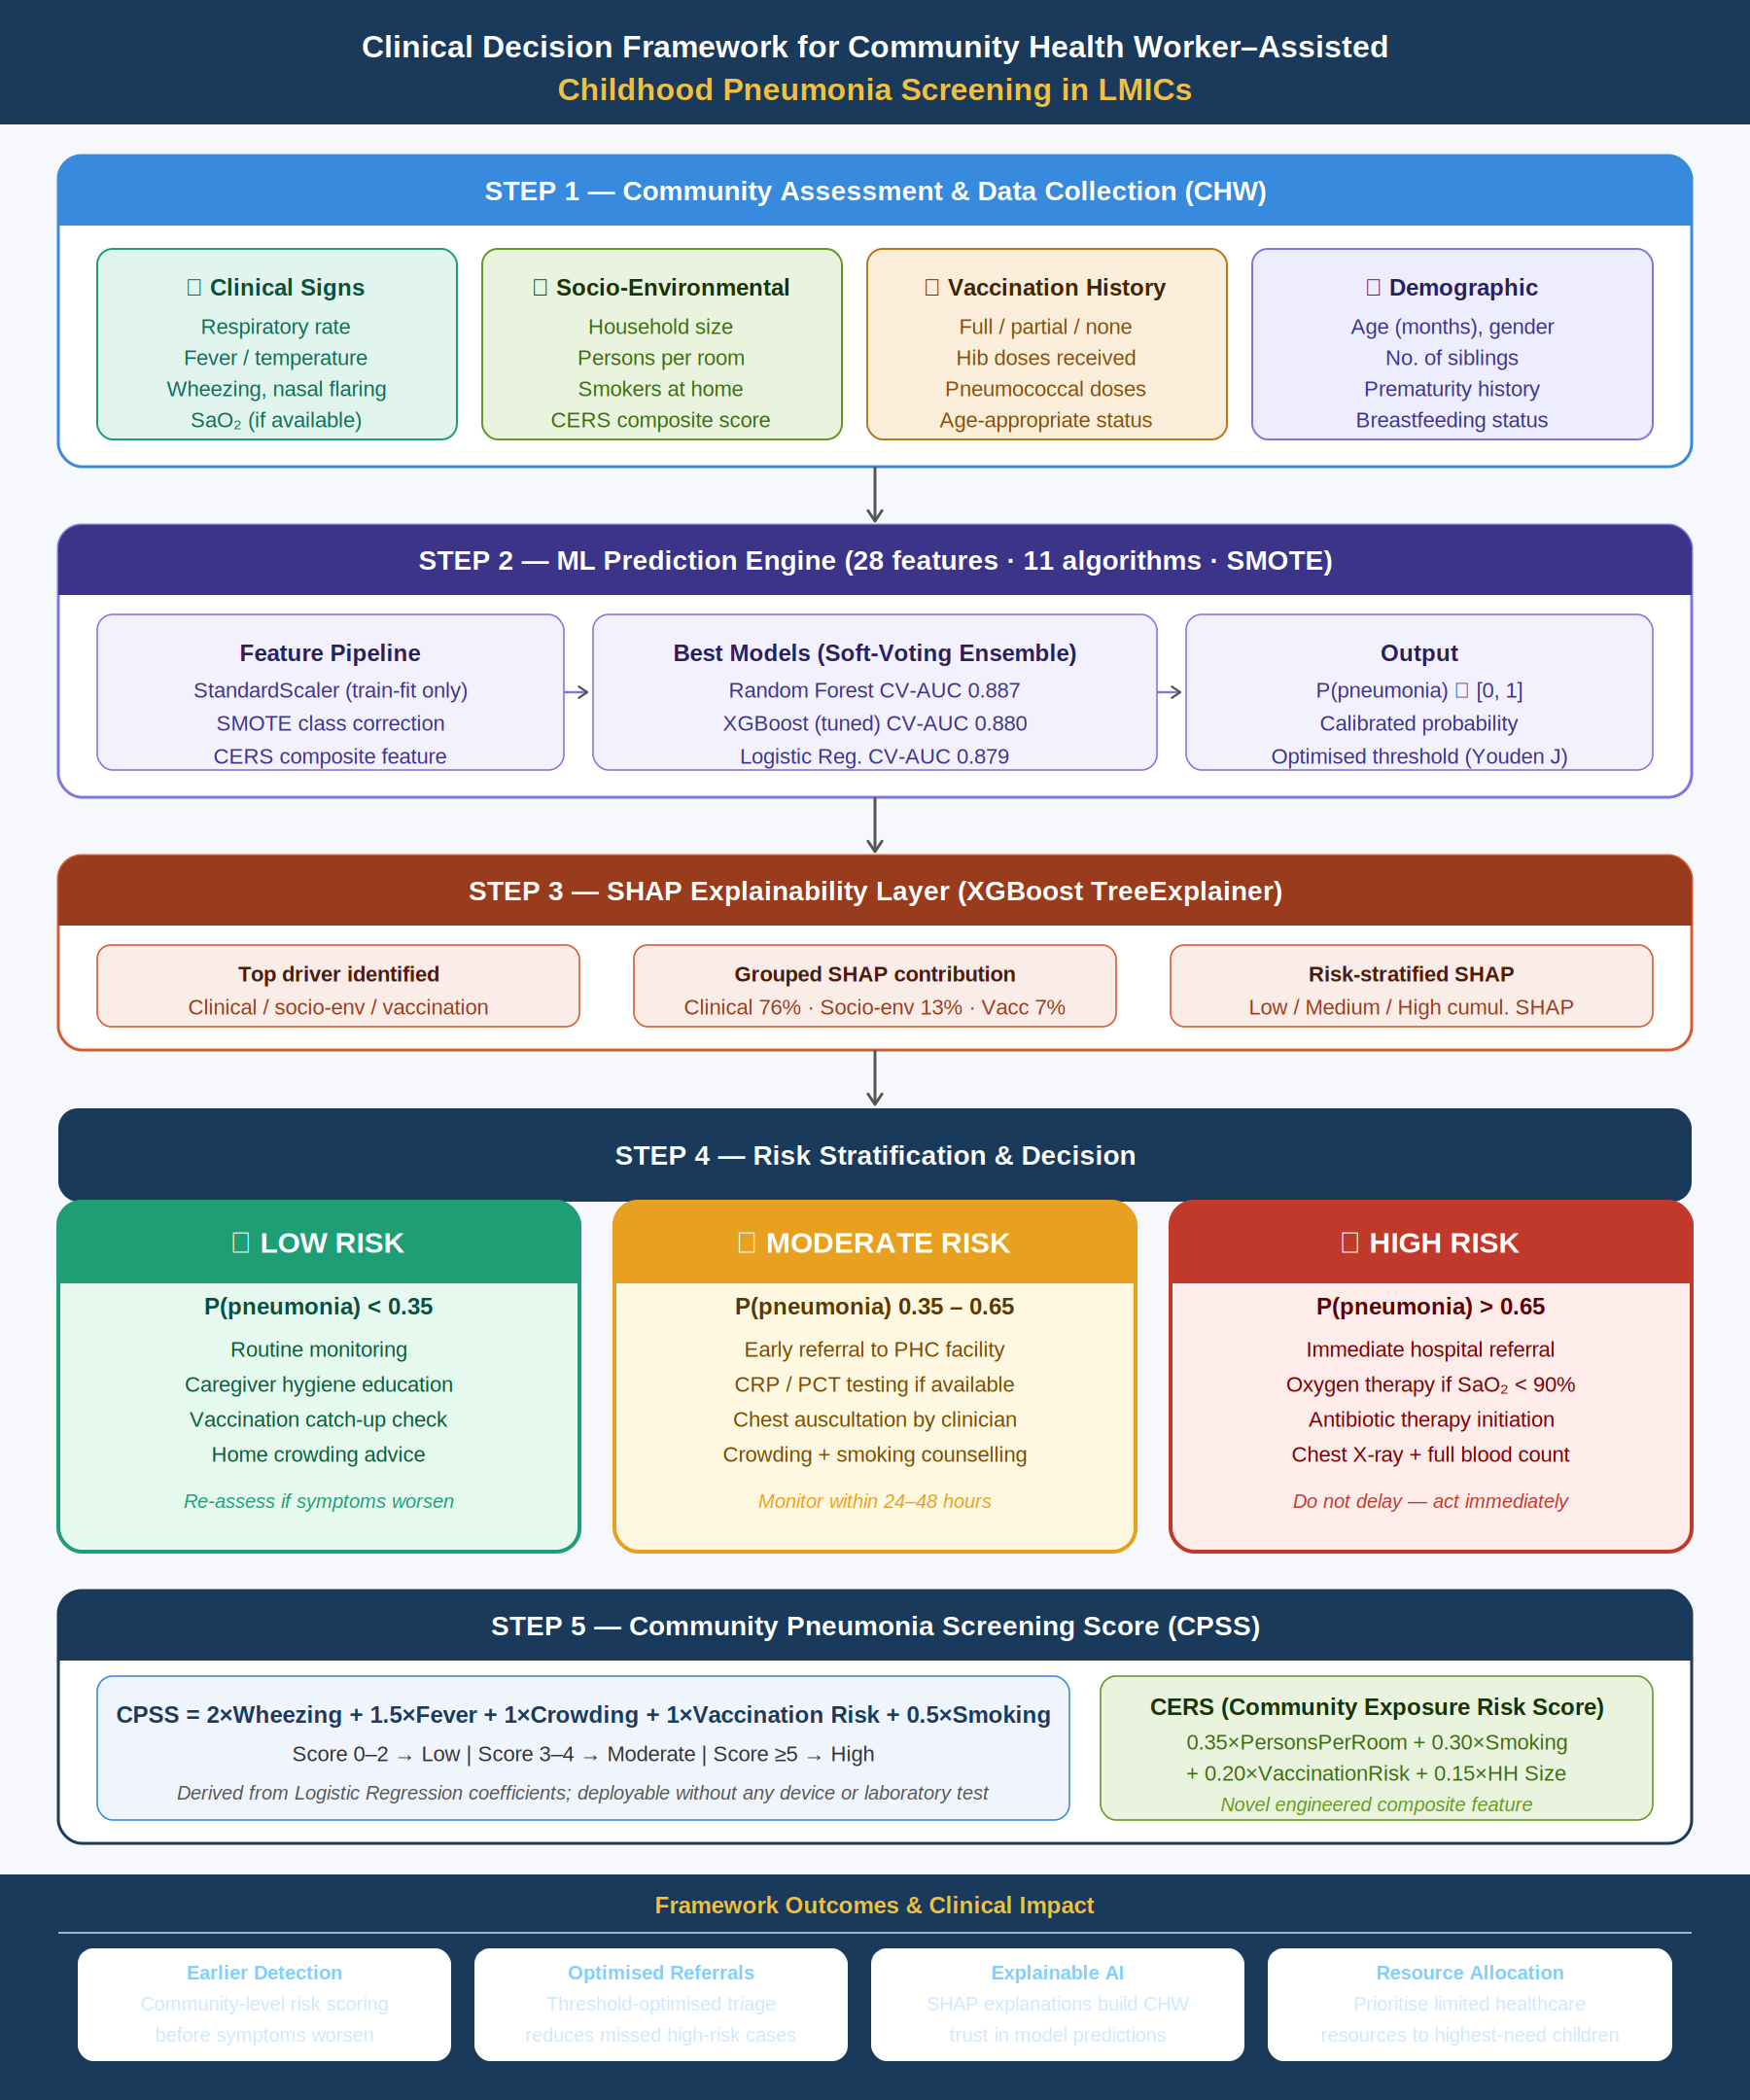
\includegraphics[width=0.92\linewidth]{figures/fig16_clinical_framework.png}
\caption{CAEPPF Clinical Decision Framework: a five-step CHW-deployable workflow from community data collection through SHAP-explained risk stratification to actionable triage.}
\label{fig:framework}
\end{figure}

\subsection{Comparison with existing literature}
Table~\ref{tab:literature} situates CAEPPF against comparable published studies.

\begin{table*}[htbp]
\centering
\caption{Comparison with existing ML studies on pediatric pneumonia.}
\label{tab:literature}
\footnotesize
\begin{tabular}{@{}llllp{6.2cm}@{}}
\toprule
Study & Best Model & Dataset & AUC & Distinction vs.\ This Study \\
\midrule
Demsash et al.\ \cite{ref6} & XGBoost & Ethiopian DHS & 0.91 & No ablation; no CERS; no calibration; no DCA; no fairness analysis \\
Serin et al.\ \cite{ref4} & Random Forest & Turkey hospital & 0.87 & Severity escalation only; no socio-env.; no SHAP; no clinical score \\
Salamon \& Ksiazek \cite{ref13} & Capsule NN & Chest X-ray & 0.97 & Imaging diagnostic, not community screening; no calibration \\
Liang \& Zheng \cite{ref14} & Deep ResNet & Chest X-ray & 0.97 & Transfer learning; requires imaging; no structured socio-env.\ features \\
\textbf{This study} & \textbf{RF + XGB ensemble} & \textbf{Morocco ($n=799$)} & \textbf{0.891} & Ablation; CERS optimization; DeLong/McNemar; calibration; DCA; fairness; SHAP dependence; CPSS; clinical framework \\
\bottomrule
\end{tabular}
\end{table*}

CAEPPF approaches the AUC of Demsash et al.\ (0.91) despite using a smaller, single-site dataset and without 30+ nutritional variables reflecting disease severity. It exceeds Serin et al.\ (0.87) while addressing a harder prediction task (community-level screening vs.\ in-hospital severity escalation). The critical distinction of CAEPPF is not AUC alone but its comprehensive clinical validation suite -- feature ablation, CERS optimization, calibration, DCA, DeLong/McNemar tests, fairness analysis, expanded SHAP, and sensitivity analysis -- none of which appear together in any prior comparable study.

%======================================================================
\section{Limitations}
%======================================================================
\begin{itemize}
\item \textbf{External generalizability:} Single tertiary care centre in Rabat, Morocco ($n=799$). Multi-site external validation across diverse LMIC populations is the highest priority next step before deployment.
\item \textbf{CERS weight derivation:} Optimized CERS weights were derived from logistic regression on the same dataset used for model training, creating a risk of circular optimism. Prospective weight validation in an independent cohort is required.
\item \textbf{Passive smoking measurement:} Binary self-report captures presence but not intensity or duration, limiting discriminatory power.
\item \textbf{Fairness subgroup sizes:} The Not Fully Vaccinated subgroup ($n=21$) is too small for reliable subgroup AUC estimation.
\item \textbf{Temporal validation:} Train--test splits are stratified but random, not time-ordered.
\item \textbf{Prospective CPSS validation:} The CPSS has not been prospectively evaluated with CHWs.
\item \textbf{Dataset size:} With 799 patients and 218 positive cases, the dataset is appropriate for exploratory ML research but at the lower end for confident subgroup analysis and calibration assessment.
\end{itemize}

%======================================================================
\section{Conclusion}
%======================================================================
This paper presented CAEPPF, the Community-Aware Explainable Pneumonia Prediction Framework, a comprehensive, clinically validated ML framework for childhood pneumonia prevalence prediction in LMIC settings, incorporating nine methodological contributions absent from prior comparable studies.

The feature ablation study provides quantitative evidence that socio-environmental variables add +1.8 AUC points over a clinical biomarker baseline, and the complete 28-feature model achieves CV-AUC~=~0.887. Data-driven CERS optimization reveals that VaccinationRisk (weight~=~0.551) is the dominant socio-environmental predictor in this cohort, substantially outweighing PersonsPerRoom -- a finding that challenges conventional epidemiological weighting assumptions and highlights the value of data-driven feature construction.

DeLong and McNemar tests confirm statistical equivalence of all top models, shifting model selection to secondary criteria: calibration, interpretability, and deployment context. Random Forest is the best-calibrated model and is recommended for probability-based triage. Decision Curve Analysis confirms all top models provide positive net benefit over default clinical strategies. Fairness analysis demonstrates consistent performance across demographic subgroups with no catastrophic failure in any group. Sensitivity analysis across ten random seeds confirms result stability.

The CPSS scoring system and five-step Clinical Decision Framework translate these findings into a CHW-deployable tool requiring no laboratory or computational infrastructure, enabling community-level pneumonia risk stratification in the resource-constrained settings where the childhood pneumonia burden is greatest. Future work should prioritize multi-site external validation, prospective CPSS evaluation with CHWs, formal calibration-based threshold optimization, and expansion of the framework to multi-disease respiratory risk prediction.

%======================================================================
\section*{CRediT authorship contribution statement}
%======================================================================
\textbf{Md Artad Chowdhury:} Conceptualization, Methodology, Software, Formal analysis, Writing -- original draft. \textbf{Bishal Paul:} Data curation, Validation, Writing -- review \& editing.

\section*{Declaration of competing interest}
The authors declare that they have no known competing financial interests or personal relationships that could have appeared to influence the work reported in this paper.

\section*{Data availability}
The dataset analyzed is publicly available via Mendeley Data (DOI: 10.17632/2d9dvnycjw.1) under a CC~BY~4.0 license \cite{ref15}.

%======================================================================
\bibliographystyle{elsarticle-num}
\bibliography{references}

\end{document}
